% !TeX program = lualatex
% このファイルは LuaLaTeX で処理してください(pdfLaTeX/upLaTeXでは動作しません)。
% Overleaf: Menu → Compiler を「LuaLaTeX」に設定
\documentclass[a4paper,11pt]{ltjsarticle}

% ========================= パッケージ =========================
\usepackage{amsmath,amssymb,mathtools}
\usepackage{ascmac}
\usepackage{comment}
\usepackage{siunitx}
\usepackage{geometry}
\usepackage{url}
\usepackage{graphicx}
\geometry{a4paper,top=15mm,bottom=18mm,left=14mm,right=14mm}
\usepackage{tikz}
\usepackage{pgfplots}
\pgfplotsset{compat=1.18}
\usepgfplotslibrary{groupplots}
\usetikzlibrary{arrows.meta,positioning,calc,patterns}
\usepackage{tcolorbox}
\usepackage{booktabs}
\usepackage{array}
\usepackage{multirow}
\usepackage{enumitem}
\usepackage{multicol}

\setlength{\parindent}{0pt}
\setlength{\parskip}{2pt}
\renewcommand{\arraystretch}{1.25}

% ========================= カスタムボックス =========================
\newtcolorbox{formulabox}[1][]{%
  colback=white,colframe=black,boxrule=1pt,arc=1.5mm,
  left=8pt,right=8pt,top=6pt,bottom=6pt,#1}
\newtcolorbox{pointbox}[1][]{%
  colback=black!4,colframe=black,boxrule=0.6pt,arc=1mm,
  left=6pt,right=6pt,top=4pt,bottom=4pt,#1}
\newtcolorbox{cautionbox}[1][]{%
  colback=white,colframe=black,boxrule=1.3pt,arc=1mm,
  left=6pt,right=6pt,top=4pt,bottom=4pt,#1}
\newtcolorbox{defbox}[1][]{%
  colback=black!3,colframe=black,boxrule=0.6pt,arc=1mm,
  left=6pt,right=6pt,top=4pt,bottom=4pt,#1}
\newtcolorbox{examplebox}[1][]{%
  colback=white,colframe=black,boxrule=0.9pt,arc=1mm,
  left=6pt,right=6pt,top=4pt,bottom=4pt,#1}

\newcommand{\banner}[1]{%
  \begin{tcolorbox}[colback=black,coltext=white,boxrule=0pt,sharp corners,
    left=8pt,right=8pt,top=5pt,bottom=5pt,before skip=8pt,after skip=8pt]
    {\Large\bfseries #1}
  \end{tcolorbox}}

\newcommand{\subbanner}[1]{%
  \begin{tcolorbox}[colback=black!85,coltext=white,boxrule=0pt,sharp corners,
    left=6pt,right=6pt,top=3pt,bottom=3pt,before skip=6pt,after skip=5pt]
    {\bfseries #1}
  \end{tcolorbox}}

\newcommand{\Meaning}[1]{%
  \begin{center}
  $\Downarrow$\\[2pt]
  {\small #1}
  \end{center}}

\pagestyle{plain}

\begin{document}

% ========================================================================
% 表紙代わりのヘッダー
% ========================================================================


\begin{center}
{\Huge\bfseries 物理基礎　波}\\[4pt]
{\Large 音の性質・弦と気柱の固有振動}\\[8pt]
\rule{\textwidth}{0.8pt}
\end{center}
\vspace{2mm}

\noindent

\vspace{3mm}


\banner{1. 音とは}

音源が振動すると，まわりの気体の\textbf{密度が周期的に変化}し，それが次々と伝わる。

\begin{center}
\begin{tikzpicture}[scale=1.0]
  % 音源(振動する膜)
  \draw[very thick] (-0.3,-0.6) -- (-0.3,0.6);
  \draw[<->,thick] (-0.6,-0.8) -- (0,-0.8);
  \node at (-0.6,1.0) {\footnotesize 音源(振動)};
  % 疎密波の粒子列
  \def\N{55}
  \def\dx{0.12}
  \def\A{0.045}
  \def\lam{1.0}
  \foreach \i in {0,...,\N}{
    \pgfmathsetmacro{\xzero}{\i*\dx}
    \pgfmathsetmacro{\xdisp}{\xzero + \A*sin(2*180*\xzero/\lam)}
    \fill (\xdisp,0) circle (1.1pt);
  }
  \draw[-{Latex[length=3mm]},thick] (0,-1.0) -- (6.2,-1.0);
  \node[right] at (3,-1.5) {\footnotesize 音波が伝わる向き};
  \node at (1.0,0.5) {\footnotesize 疎};
  \node at (1.5,0.5) {\footnotesize 密};
  \node at (2.0,0.5) {\footnotesize 疎};
  \node at (2.5,0.5) {\footnotesize 密};
\end{tikzpicture}
\end{center}

\begin{defbox}
\textbf{音波}：振動する物体（音源）が周囲の空気分子を押し縮めたり引き離したりすることで，エネルギーが縦波として伝播する現象\\
\textbf{音源}：音を発する物体。
\end{defbox}

\begin{cautionbox}
\boxed{\text{注意}}\quad 音波は\textbf{媒質がなければ伝わらない}。真空中では音は聞こえない。
\end{cautionbox}

% ------------------------------------------------------------------
\subbanner{音の速さ(音速)}

音速は\textbf{媒質によって決まり，振動数や振幅にはよらない}。

\begin{formulabox}
\begin{center}
\textbf{温度と音の速さ(乾燥空気中)}\\[4pt]
$\boxed{\,V = 331.5 + 0.6\,t\,}$\\[4pt]
{\footnotesize $V$：音の速さ[m/s]\quad $t$：摂氏温度[$\si{\celsius}$]}
\end{center}
\end{formulabox}
\begin{center}
\begin{tabular}{@{}lllr@{}}
\toprule
状態 & 媒質 & 温度 & 音速[m/s] \\
\midrule
\multirow[t]{3}{*}{気体中} & 二酸化炭素 & \SI{0}{\celsius} & 258 \\
 & 乾燥空気 & \SI{0}{\celsius} & 331.5 \\
 & ヘリウム & \SI{0}{\celsius} & 970 \\
\midrule
\multirow[t]{3}{*}{液体中} & エタノール & \SI{23}{\celsius}～\SI{27}{\celsius} & 1207 \\
 & 蒸留水 & \SI{23}{\celsius}～\SI{27}{\celsius} & 1500 \\
 & 海水 & \SI{20}{\celsius} & 1513 \\
\midrule
\multirow[t]{2}{*}{固体中} & 鉄 & --- & 5950 \\
 & アルミニウム & --- & 6420 \\
\bottomrule
\end{tabular}
\end{center}



\clearpage
% ========================================================================
\banner{2. 音の3要素}

同じ音源からの音でも，「大きさ」「高さ」「音色」という3つの独立な物理量で特徴づけられる。

\begin{center}
\begin{tikzpicture}
\begin{groupplot}[
  group style={group size=1 by 3, vertical sep=0.7cm},
  height=2.6cm, width=9.5cm,
  xmin=0,xmax=2,ymin=-1.6,ymax=1.6,
  xtick=\empty, ytick=\empty, axis lines=middle,
  title style={font=\footnotesize},
]
\nextgroupplot[title={音の大きさ $\leftrightarrow$ 振幅}]
\addplot[domain=0:2,samples=60,thick] {1.3*sin(360*2*x)};
\addplot[domain=0:2,samples=60,thick,dashed] {0.5*sin(360*2*x)};
\nextgroupplot[title={音の高さ $\leftrightarrow$ 振動数}]
\addplot[domain=0:2,samples=80,thick] {1*sin(360*5*x)};
\addplot[domain=0:2,samples=60,thick,dashed] {1*sin(360*2*x)};
\nextgroupplot[title={音色 $\leftrightarrow$ 波形}]
\addplot[domain=0:2,samples=80,thick] {sin(360*3*x)};
\addplot[domain=0:2,samples=80,thick,dashed] {sin(360*3*x)+0.35*sin(360*9*x+40)};
\end{groupplot}
\end{tikzpicture}
\end{center}
\begin{center}
{\footnotesize (実線・破線はそれぞれ「音が大きい／小さい」「音が高い／低い」「楽器Aの音／楽器Bの音」を表す)}
\end{center}


\begin{center}
\begin{tabular}{@{}lll@{}}
\toprule
音の3要素 & 対応する物理量 & 変化の様子 \\
\midrule
音の\textbf{大きさ} & 振幅 & 振幅が大きくなる $\Rightarrow$ 音は大きくなる \\
音の\textbf{高さ} & 振動数 & 振動数が大きくなる $\Rightarrow$ 音は高くなる \\
\textbf{音色} & 波形 & 波形が違う $\Rightarrow$ 音色が違う \\
\bottomrule
\end{tabular}
\end{center}


\begin{defbox}
\textbf{可聴音}：ヒトが聞こえる音の振動数はおよそ $\SI{200}{Hz}$～$\SI{20000}{Hz}$。\\
\textbf{超音波}：$\SI{20000}{Hz}$ をこえる振動数の音波。
\end{defbox}


\clearpage
% ========================================================================
\banner{3. うなり}

振動数がわずかに異なる2つの音を同時に鳴らすと，音の大きさが周期的に変化する「ウァーン，ウァーン」という現象が聞こえる。

\begin{center}
\begin{tikzpicture}
\begin{groupplot}[
  group style={group size=1 by 3, vertical sep=0.55cm},
  width=11cm,height=2.7cm,
  xmin=0,xmax=2,ymin=-2.3,ymax=2.3,
  xtick=\empty, ytick=\empty, axis lines=middle,
  title style={font=\footnotesize},
]
\nextgroupplot[title={振動数 $f_1$ のおんさ}]
\addplot[domain=0:2,samples=80,thick]{sin(360*6*x)};
\nextgroupplot[title={振動数 $f_2$ のおんさ}]
\addplot[domain=0:2,samples=80,thick]{sin(360*5*x)};
\nextgroupplot[title={重なり合った音波(うなり)}]
\addplot[domain=0:2,samples=150,thick]{sin(360*6*x)+sin(360*5*x)};
\addplot[domain=0:2,samples=50,dashed]{
  2*cos(360*0.5*x)};
\addplot[domain=0:2,samples=50,dashed]{-2*cos(360*0.5*x)};
\draw[<->] (axis cs:0,-2.1) -- (axis cs:2,-2.1) node[midway,below,font=\scriptsize]{うなりの周期 $T_0$};
\end{groupplot}
\end{tikzpicture}
\end{center}

\begin{formulabox}
\begin{center}
\textbf{1秒間あたりのうなりの回数}\\[4pt]
$\boxed{\,f = \dfrac{1}{T_0} = |f_1 - f_2|\,}$\\[4pt]
{\footnotesize $f$：1秒間あたりのうなりの回数\quad $T_0$：うなりの周期\quad $f_1,f_2$：2つの音の振動数}
\end{center}
\end{formulabox}

\Meaning{2つの振動数の\textbf{差の絶対値}が，1秒間に感じるうなりの回数になる}

\begin{pointbox}
$f_1$ と $f_2$ の差が小さいほど，うなりはゆっくり(回数は少なく)なる。差が0になるとうなりは消える $\to$ \textbf{楽器の調律}に利用される。
\end{pointbox}

\begin{examplebox}
\textbf{コラム：ピアノの調律と平均律}\\
ピアノの調律では，単にうなりを消すのではなく，\textbf{規定の回数のうなりが生じるように}調律する。ここで使われる「平均律」とは，1オクターブ(振動数2倍)を鍵盤12個分に均等に割り振った音律である。$\to$ 次ページで数式化する。
\end{examplebox}

\clearpage

\banner{【発展】音階}

\subbanner{オクターブと平均律}

音響学において，1オクターブ高い音とは元の音のちょうど2倍の周波数の音であると定義されている。我々がよく耳にするド ド\#  レ ミ ファ ファ\# ソ ソ\# ラ ラ\# シ ドという音階は，1オクターブを半音12個に均等分割したものである。

\begin{defbox}
\textbf{平均律}：隣り合う鍵盤の振動数の比が常に一定になるように，1オクターブ(比2倍)を等分した音律。
\end{defbox}

半音 $n$ 個上の振動数を $f_n$，基準の振動数を $f_0$，隣り合う半音の振動数比を $r$ とすると，$f_n=f_0 r^n$。$n=12$ で2倍になることから $r^{12}=2$，すなわち $r=2^{1/12}$。

\begin{itembox}[l]{12平均律における振動数}
\begin{center}
$\boxed{\,f_n = f_0\cdot 2^{\,n/12}\,}$\\[4pt]
{\footnotesize $f_n$：基準音から半音 $n$ 個上の振動数\quad $f_0$：基準音の振動数\quad $n$：半音の数(整数)}
\end{center}
\end{itembox}

両辺の底2の対数をとると，

\[
n = 12\log_2\!\left(\dfrac{f_n}{f_0}\right)
\]
→2つの音が半音でいくつ違うかを知りたいときは2つの音の周波数と対数によって求まる。

\subbanner{音階と振動数の対応表}
ここで，基準音を$f_0=440[\mathrm{Hz}]$と設定\footnote{ピアノやリコーダーなどはA4$=442[\mathrm{Hz}]$で調律されていることが多いので注意}
し，この音階をA4（hiAともいう）とすると，$\boxed{f_n=440\cdot 2^{n/12}}$ より，C3からB7までの各音の振動数が下の表のように求まる。
\begin{center}
{\footnotesize
\begin{tabular}{@{}c*{12}{r}@{}}
\toprule
\textbf{オクターブ} & C & C\# & D & D\# & E & F & F\# & G & G\# & A & A\# & B \\
\midrule
3 & 130.8 & 138.6 & 146.8 & 155.6 & 164.8 & 174.6 & 185.0 & 196.0 & 207.7 & 220.0 & 233.1 & 246.9 \\
4 & 261.6 & 277.2 & 293.7 & 311.1 & 329.6 & 349.2 & 370.0 & 392.0 & 415.3 & 440.0 & 466.2 & 493.9 \\
5 & 523.3 & 554.4 & 587.3 & 622.3 & 659.3 & 698.5 & 740.0 & 784.0 & 830.6 & 880.0 & 932.3 & 987.8 \\
6 & 1046.5 & 1108.7 & 1174.7 & 1244.5 & 1318.5 & 1396.9 & 1480.0 & 1568.0 & 1661.2 & 1760.0 & 1864.7 & 1975.5 \\
7 & 2093.0 & 2217.5 & 2349.3 & 2489.0 & 2637.0 & 2793.8 & 2960.0 & 3136.0 & 3322.4 & 3520.0 & 3729.3 & 3951.1 \\
\bottomrule
\end{tabular}
}
\end{center}
\begin{center}
{\footnotesize 単位は $\mathrm{Hz}$。基準音 $f_0=\SI{440}{Hz}$(A4)としたときの平均律による値。}
\end{center}

\clearpage
\subbanner{【超発展】和音と周期}
1オクターブ違う2つの音を同じ種類の音であると感じたり，特定の和音を美しく(協和的に)感じたりするのは，2つの音を重ね合わせたときにできる波の形が単純で規則的になるためである。振動数の比が簡単な整数比になっていると，波の「山」の位置が短い間隔で重なり合い，全体として滑らかな波形になる。これが「協和音」として心地よく聞こえる理由である。

% ---------------- 完全5度 ----------------
\begin{figure}[htbp]
\centering
\begin{tikzpicture}
\begin{axis}[
    width=11cm, height=5cm,
    title={完全5度　周波数比 3:2},
    xlabel={$t$（任意時間単位）}, ylabel={振幅},
    xmin=0, xmax=1, ymin=-1.2, ymax=1.2,
    legend style={font=\scriptsize}, legend pos=outer north east,
]
\addplot[domain=0:1,samples=200,thick,blue] {sin(2*360*x)};
\addplot[domain=0:1,samples=200,thick,red]  {sin(3*360*x)};
\legend{根音(2), 上音(3)}
\end{axis}
\end{tikzpicture}
\caption{完全5度の波形（周期数 2:3，1周期ごとには一致しないが3周期ごとに一致する）}
\end{figure}

% ---------------- 完全8度 ----------------
\begin{figure}[htbp]
\centering
\begin{tikzpicture}
\begin{axis}[
    width=11cm, height=5cm,
    title={完全8度（オクターブ）　周波数比 2:1},
    xlabel={$t$（任意時間単位）}, ylabel={振幅},
    xmin=0, xmax=1, ymin=-1.2, ymax=1.2,
    legend style={font=\scriptsize}, legend pos=outer north east,
]
\addplot[domain=0:1,samples=200,thick,blue] {sin(1*360*x)};
\addplot[domain=0:1,samples=200,thick,red]  {sin(2*360*x)};
\legend{根音(1), 上音(2)}
\end{axis}
\end{tikzpicture}
\caption{完全8度の波形（周期数 1:2，1周期ごとに完全一致）}
\end{figure}

% ---------------- 短2度（不協和音の例） ----------------
\begin{figure}[htbp]
\centering
\begin{tikzpicture}
\begin{axis}[
    width=11cm, height=5cm,
    title={短2度　周波数比 $2^{1/12}:1\approx1.06:1$（不協和）},
    xlabel={$t$（任意時間単位）}, ylabel={振幅},
    xmin=0, xmax=4, ymin=-1.2, ymax=1.2,
    legend style={font=\scriptsize}, legend pos=outer north east,
]
\addplot[domain=0:4,samples=400,thick,blue] {sin(1*360*x)};
\addplot[domain=0:4,samples=400,thick,red]  {sin(2^(1/12)*360*x)};
\legend{根音(1), 上音($2^{1/12}$)}
\end{axis}
\end{tikzpicture}
\caption{短2度の波形。山の位置がなかなかそろわず，波形がいつまでも複雑なまま}
\end{figure}



\clearpage
\banner{【復習】定在波}

同じ振幅$A$，波長$\lambda$をもつ2つの波が，互いに\textbf{逆向き}に進んで重なると，波形全体は左右に移動せず，その場で振幅だけが周期的に変化する波ができる。これを\textbf{定在波(定常波)}という。
定在波は，振幅・波長が等しい2つの波が逆向きに重なるとできる。弦や気柱では，\textbf{入射波と反射波}が重なることで定在波が生じる。

\begin{center}
\begin{tikzpicture}
\begin{groupplot}[
  group style={group size=1 by 3, vertical sep=0.7cm},
  width=11.5cm,height=3.4cm,
  xmin=0,xmax=3,ymin=-3.5,ymax=3.5,
  xtick=\empty, ytick=\empty, axis lines=middle,
  title style={font=\footnotesize},
  clip=false,
]
\nextgroupplot[]
\node[anchor=east,font=\scriptsize,align=right] at (axis description cs:-0.02,0.5) {$t=0$};
\addplot[gray!50,dashed,domain=0:3,samples=100]{2.8*sin(360*x)};
\addplot[gray!50,dashed,domain=0:3,samples=100]{-2.8*sin(360*x)};
\addplot[thick,domain=0:3,samples=100]{2.8*sin(360*x)};
\draw[dashed,gray,thin] (axis cs:0,-3) -- (axis cs:0,3);
\draw[dashed,gray,thin] (axis cs:0.5,-3) -- (axis cs:0.5,3);
\draw[dashed,gray,thin] (axis cs:1,-3) -- (axis cs:1,3);
\draw[dashed,gray,thin] (axis cs:1.5,-3) -- (axis cs:1.5,3);
\draw[dashed,gray,thin] (axis cs:2,-3) -- (axis cs:2,3);
\draw[dashed,gray,thin] (axis cs:2.5,-3) -- (axis cs:2.5,3);
\draw[dashed,gray,thin] (axis cs:3,-3) -- (axis cs:3,3);
\draw[dashed,gray,thin] (axis cs:0.25,-3) -- (axis cs:0.25,3);
\draw[dashed,gray,thin] (axis cs:0.75,-3) -- (axis cs:0.75,3);
\draw[dashed,gray,thin] (axis cs:1.25,-3) -- (axis cs:1.25,3);
\draw[dashed,gray,thin] (axis cs:1.75,-3) -- (axis cs:1.75,3);
\draw[dashed,gray,thin] (axis cs:2.25,-3) -- (axis cs:2.25,3);
\draw[dashed,gray,thin] (axis cs:2.75,-3) -- (axis cs:2.75,3);
\node[font=\scriptsize] at (axis cs:0,3.9) {節};
\node[font=\scriptsize] at (axis cs:0.5,3.9) {節};
\node[font=\scriptsize] at (axis cs:1,3.9) {節};
\node[font=\scriptsize] at (axis cs:1.5,3.9) {節};
\node[font=\scriptsize] at (axis cs:2,3.9) {節};
\node[font=\scriptsize] at (axis cs:2.5,3.9) {節};
\node[font=\scriptsize] at (axis cs:3,3.9) {節};
\node[font=\scriptsize] at (axis cs:0.25,3.9) {腹};
\node[font=\scriptsize] at (axis cs:0.75,3.9) {腹};
\node[font=\scriptsize] at (axis cs:1.25,3.9) {腹};
\node[font=\scriptsize] at (axis cs:1.75,3.9) {腹};
\node[font=\scriptsize] at (axis cs:2.25,3.9) {腹};
\node[font=\scriptsize] at (axis cs:2.75,3.9) {腹};
\draw[<->] (axis cs:0,-3.3) -- (axis cs:0.5,-3.3) node[midway,below,font=\scriptsize]{$\lambda/2$(節と節)};


\nextgroupplot[]
\node[anchor=east,font=\scriptsize,align=right] at (axis description cs:-0.02,0.5) {$t=T/4$\\全体が一瞬 $y=0$};
\addplot[gray!50,dashed,domain=0:3,samples=100]{2.8*sin(360*x)};
\addplot[gray!50,dashed,domain=0:3,samples=100]{-2.8*sin(360*x)};
\addplot[thick,domain=0:3,samples=10]{0*x};
\draw[dashed,gray,thin] (axis cs:0,-3) -- (axis cs:0,3);
\draw[dashed,gray,thin] (axis cs:0.5,-3) -- (axis cs:0.5,3);
\draw[dashed,gray,thin] (axis cs:1,-3) -- (axis cs:1,3);
\draw[dashed,gray,thin] (axis cs:1.5,-3) -- (axis cs:1.5,3);
\draw[dashed,gray,thin] (axis cs:2,-3) -- (axis cs:2,3);
\draw[dashed,gray,thin] (axis cs:2.5,-3) -- (axis cs:2.5,3);
\draw[dashed,gray,thin] (axis cs:3,-3) -- (axis cs:3,3);
\draw[dashed,gray,thin] (axis cs:0.25,-3) -- (axis cs:0.25,3);
\draw[dashed,gray,thin] (axis cs:0.75,-3) -- (axis cs:0.75,3);
\draw[dashed,gray,thin] (axis cs:1.25,-3) -- (axis cs:1.25,3);
\draw[dashed,gray,thin] (axis cs:1.75,-3) -- (axis cs:1.75,3);
\draw[dashed,gray,thin] (axis cs:2.25,-3) -- (axis cs:2.25,3);
\draw[dashed,gray,thin] (axis cs:2.75,-3) -- (axis cs:2.75,3);

\nextgroupplot[]
\node[anchor=east,font=\scriptsize,align=right] at (axis description cs:-0.02,0.5) {$t=T/2$};
\addplot[gray!50,dashed,domain=0:3,samples=100]{2.8*sin(360*x)};
\addplot[gray!50,dashed,domain=0:3,samples=100]{-2.8*sin(360*x)};
\addplot[thick,domain=0:3,samples=100]{-2.8*sin(360*x)};
\draw[dashed,gray,thin] (axis cs:0,-3) -- (axis cs:0,3);
\draw[dashed,gray,thin] (axis cs:0.5,-3) -- (axis cs:0.5,3);
\draw[dashed,gray,thin] (axis cs:1,-3) -- (axis cs:1,3);
\draw[dashed,gray,thin] (axis cs:1.5,-3) -- (axis cs:1.5,3);
\draw[dashed,gray,thin] (axis cs:2,-3) -- (axis cs:2,3);
\draw[dashed,gray,thin] (axis cs:2.5,-3) -- (axis cs:2.5,3);
\draw[dashed,gray,thin] (axis cs:3,-3) -- (axis cs:3,3);
\draw[dashed,gray,thin] (axis cs:0.25,-3) -- (axis cs:0.25,3);
\draw[dashed,gray,thin] (axis cs:0.75,-3) -- (axis cs:0.75,3);
\draw[dashed,gray,thin] (axis cs:1.25,-3) -- (axis cs:1.25,3);
\draw[dashed,gray,thin] (axis cs:1.75,-3) -- (axis cs:1.75,3);
\draw[dashed,gray,thin] (axis cs:2.25,-3) -- (axis cs:2.25,3);
\draw[dashed,gray,thin] (axis cs:2.75,-3) -- (axis cs:2.75,3);
\draw[<->] (axis cs:0,-3.9) -- (axis cs:1,-3.9) node[midway,below,font=\scriptsize]{$\lambda$};
\end{groupplot}
\end{tikzpicture}
\end{center}

\begin{defbox}
\textbf{節(node)}：常に $y=0$ で静止している点。\\
\textbf{腹(antinode)}：最も大きく振動する点(振幅 $2A$)。
\end{defbox}
\begin{defbox}
\textbf{節と節の距離}(または\textbf{腹と腹の距離})：$\dfrac{\lambda}{2}$\\
\textbf{節と腹の距離}：$\dfrac{\lambda}{4}$
\end{defbox}





\clearpage




\banner{4. 弦の固有振動}
\subbanner{固有振動}
単振り子の周期は，振れ幅が小さいとき，長さ$l$にのみ依存し，その値は$T = \sqrt{\frac{l}{g}}$であった。\footnote{振り子時計はこの仕組みを利用している}（$g$：重力加速度）
一般に，ある物体を振動させると，物体はその材質や形状によって決まる特定の振動数で振動する。この振動を\textbf{固有振動}といい，この時の振動数を\textbf{固有振動数}という。
\subbanner{共振（共鳴）}
物体のもつ固有振動数と同じ振動数の振動を与えると，その物体は振動しはじめ，やがて大きな振動となる。この現象を\textbf{共振(共鳴)}という。\footnote{共振と共鳴は同じ意味だが，空気を仲立ちとして音が出るときは共鳴と呼ぶことが多い。}
\subbanner{弦の固有振動(両端が節)}
ギターの弦をはじくと決まった高さの音が出るように弦にも固有振動が存在し，そこには\textbf{定在波}ができている。つまり，腹と節が存在する。
弦の両端は固定されているため，定在波の\textbf{節}になる。弦の長さを $L$，弦を伝わる波の速さを $v$ とする。

\begin{center}
\renewcommand{\arraystretch}{2.6}
\begin{tabular}{cc|c|c}
\cline{2-4} % 表部分（2〜4列目）の上側の罫線。弦の図の列には引かない

% ---- ヘッダー行 ----
\makebox[3.6cm][l]{\hspace{-1.2cm}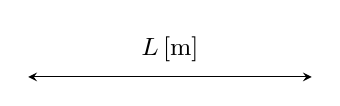
\begin{tikzpicture}[x=1cm,y=1cm]
  \draw[<->,>=stealth] (0,0) -- (3.6,0); % 弦全体の長さ L を示す両矢印
  \node[font=\small] at (1.8,0.35) {$L\,[\mathrm{m}]$}; % 矢印の上に長さのラベルを表示
\end{tikzpicture}}
& % 振動の名称列（ヘッダー行なので空欄）
& \textbf{波長 $\lambda\,[\mathrm{m}]$} % 波長列の見出し
& \textbf{振動数 $f\,[\mathrm{Hz}]$} \\ % 振動数列の見出し
\cline{2-4} % ヘッダー行の下側の罫線（弦の図の列には引かない）

% ---- 基本振動 (n=1) ----
\makebox[3.6cm][l]{\hspace{-1.2cm}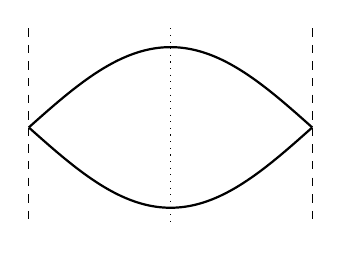
\begin{tikzpicture}[x=0.6cm,y=0.6cm]
  \draw[thick,domain=0:6,samples=60,smooth,variable=\x]
    plot ({\x},{1.7*sin(30*\x)}); % 変位の波形（上半分）
  \draw[thick,domain=0:6,samples=60,smooth,variable=\x]
    plot ({\x},{-1.7*sin(30*\x)}); % 変位の波形（下半分）
  \draw[dashed] (0,2.1) -- (0,-2.1); % 左端（固定端）にある節の位置を示す点線
  \draw[dashed] (6,2.1) -- (6,-2.1); % 右端（固定端）にある節の位置を示す点線
  \draw[dotted] (3,2.1) -- (3,-2.1); % 中央にある腹の位置を示す点線
\end{tikzpicture}}
& 基本振動 & $\lambda_1 = 2L = \dfrac{2L}{1}$ & $f_1 = \dfrac{1}{2L}v$ \\
\cline{2-4} % この行の下側の罫線

% ---- 2倍振動 (n=2) ----
\makebox[3.6cm][l]{\hspace{-1.2cm}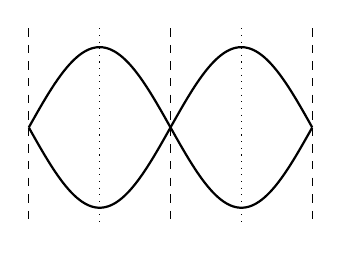
\begin{tikzpicture}[x=0.6cm,y=0.6cm]
  \draw[thick,domain=0:6,samples=60,smooth,variable=\x]
    plot ({\x},{1.7*sin(60*\x)}); % 変位の波形（上半分）
  \draw[thick,domain=0:6,samples=60,smooth,variable=\x]
    plot ({\x},{-1.7*sin(60*\x)}); % 変位の波形（下半分）
  \draw[dashed] (0,2.1) -- (0,-2.1); % 左端（固定端）にある節の位置を示す点線
  \draw[dashed] (3,2.1) -- (3,-2.1); % 中央にある節の位置を示す点線
  \draw[dashed] (6,2.1) -- (6,-2.1); % 右端（固定端）にある節の位置を示す点線
  \draw[dotted] (1.5,2.1) -- (1.5,-2.1); % 1つ目の腹の位置を示す点線
  \draw[dotted] (4.5,2.1) -- (4.5,-2.1); % 2つ目の腹の位置を示す点線
\end{tikzpicture}}
& 2倍振動 & $\lambda_2 = L = \dfrac{2L}{2}$ & $f_2 = \dfrac{2}{2L}v$ \\
\cline{2-4}

% ---- 3倍振動 (n=3) ----
\makebox[3.6cm][l]{\hspace{-1.2cm}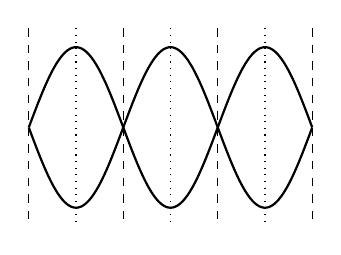
\begin{tikzpicture}[x=0.6cm,y=0.6cm]
  \draw[thick,domain=0:6,samples=60,smooth,variable=\x]
    plot ({\x},{1.7*sin(90*\x)}); % 変位の波形（上半分）
  \draw[thick,domain=0:6,samples=60,smooth,variable=\x]
    plot ({\x},{-1.7*sin(90*\x)}); % 変位の波形（下半分）
  \draw[dashed] (0,2.1) -- (0,-2.1); % 左端（固定端）の節
  \draw[dashed] (2,2.1) -- (2,-2.1); % 1つ目の内部の節
  \draw[dashed] (4,2.1) -- (4,-2.1); % 2つ目の内部の節
  \draw[dashed] (6,2.1) -- (6,-2.1); % 右端（固定端）の節
  \draw[dotted] (1,2.1) -- (1,-2.1); % 1つ目の腹
  \draw[dotted] (3,2.1) -- (3,-2.1); % 2つ目の腹
  \draw[dotted] (5,2.1) -- (5,-2.1); % 3つ目の腹
\end{tikzpicture}}
& 3倍振動 & $\lambda_3 = \dfrac{2L}{3}$ & $f_3 = \dfrac{3}{2L}v$ \\
\cline{2-4}

% ---- n倍振動（両端に2ループずつ表示、中央は「…」で省略。節の点線は付けない） ----
\makebox[3.6cm][l]{\hspace{-1.2cm}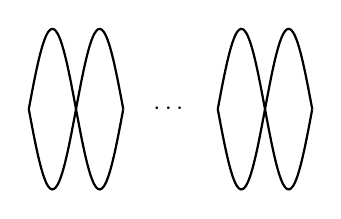
\begin{tikzpicture}[x=0.6cm,y=0.6cm]
  % 左端2ループ分の波形（上半分）
  \draw[thick,domain=0:2,samples=50,smooth,variable=\x]
    plot ({\x},{1.7*sin(180*\x)});
  % 左端2ループ分の波形（下半分）
  \draw[thick,domain=0:2,samples=50,smooth,variable=\x]
    plot ({\x},{-1.7*sin(180*\x)});
  % 右端2ループ分の波形（上半分）
  \draw[thick,domain=4:6,samples=50,smooth,variable=\x]
    plot ({\x},{1.7*sin(180*\x)});
  % 右端2ループ分の波形（下半分）
  \draw[thick,domain=4:6,samples=50,smooth,variable=\x]
    plot ({\x},{-1.7*sin(180*\x)});
  \node[font=\small] at (3,0) {$\cdots$}; % 中央部分：多数のループが続くことを省略記号で示す
\end{tikzpicture}}
& n倍振動 & $\lambda_n = \dfrac{2L}{n}$ & $f_n = \dfrac{n}{2L}v$ \\
\cline{2-4}
\end{tabular}
\end{center}



\begin{pointbox}
\textbf{弦を伝わる波の速さ}：張力 $S$[N]，線密度(単位長さあたりの質量) $\rho$[kg/m] とすると，
\[
v=\sqrt{\dfrac{S}{\rho}}
\]
張力が大きいほど，また線密度(弦の太さ)が小さいほど，$v$ は大きく，$f_1$ も大きくなる(高い音)。
\end{pointbox}

\subbanner{弦楽器のしくみ}

\begin{center}
\begin{tikzpicture}[scale=1.5]
  % ボディ(胴)：弦の高さ(y=0.7)を中心に置く
  \draw[thick,fill=black!5] (6.5,0.7) ellipse (2.3 and 2.0);
  % サウンドホール(胴に開いた穴)
  \draw[thick,fill=white] (6.0,0.7) circle (0.9);
  \node[font=\scriptsize,align=center] at (6.0,0.7) {サウンド\\ホール};
  % ネック(ボディの左端に重ねて継ぎ目をなくす)
  \draw[thick,fill=black!5] (0,0.5) rectangle (4.6,0.9);
  \foreach \x in {0.5,1.0,1.5,2.0,2.5,3.5,4.0}{\draw (\x,0.5)--(\x,0.9);}
  \node[above,font=\footnotesize] at (1.0,0.95) {フレット};
  % ペグ(糸巻き)
  \draw[thick,fill=black!20] (-0.6,0.3) rectangle (0,1.1);
  \node[left,font=\scriptsize,align=center] at (-0.7,0.7) {ペグ\\(張力調整)};
  % 弦(ボディの上に重ねて最前面に描く)
  \draw[thick] (0,0.7) -- (7.8,0.7);
  \fill (7.8,0.7) circle (1.8pt);
  % 弦の振動する長さ L の範囲(ナット～ブリッジ)
  \draw[<->] (3.0,0.15) -- (7.8,0.15) node[midway,below,font=\scriptsize]{弦の長さ $L$};
  % 押さえる指の位置
  \draw[->] (3.0,1.9) -- (3.0,0.95);
  \node[above,font=\scriptsize,align=center] at (3.0,1.95) {押さえる位置で\\弦の長さ $L$ を変える};
  \fill (3.0,0.7) circle (1.8pt);
  % キャプション
  \node[below,font=\footnotesize,align=center,text width=8.6cm] at (6.3,-1.5) {胴(共鳴胴)：弦の振動を空気の大きな振動に変え，大きな音を出す};
\end{tikzpicture}
\end{center}

\begin{pointbox}
\begin{itemize}[itemsep=1pt]
  \item ペグで\textbf{張力 $S$} を変える $\to$ 強く張るほど高い音
  \item フレットで\textbf{弦の長さ $L$} を変える $\to$ 短いほど高い音($f_1=v/2L$)
  \item 弦の太さ($\rho$)が細いほど高い音
  \item 実際の弦の振動は基本振動と倍振動が混ざり合ったもの $\to$ 混じり方の違いが\textbf{音色}の違いを生む
\end{itemize}
\end{pointbox}

\clearpage
\banner{5. 気柱の固有振動}
\subbanner{共鳴と固有振動数}
ギターの弦をはじくと決まった高さの音が出るように気柱にも固有振動が存在し，
そこには定在波ができていた。
リコーダーなどの管楽器は同じ押さえ方をすると同じ音がでるように，弦にも固有振動が存在し，そこには\textbf{定在波}ができている。\\
\subbanner{閉管と開管}

管の一方の端が閉じているものを\textbf{閉管}，両端が開いているものを\textbf{開管}という。
\begin{center}
\begin{tikzpicture}[x=1cm,y=1cm,>=stealth]

  % ------- 列見出し：開管／閉管 -------
  \node[font=\bfseries\large] at (2.5,5.2) {開管};
  \node[font=\bfseries\large] at (10.0,5.2) {閉管};


  %================= 上段：3D表示 =================

  % ---- 左列：開管（両端が開いている）の3D図 ----
  \begin{scope}[shift={(0,3.6)}]
    \draw[thick] (0,0.9) -- (5,0.9);
    \draw[thick] (0,-0.9) -- (5,-0.9);
    \draw[thick] (0,0) ellipse (0.3 and 0.9);                          % 左：完全に開いた口
    \draw[thick,dashed] (5,0.9) arc (90:270:0.3 and 0.9);              % 右：手前側(破線)
    \draw[thick] (5,0.9) arc (90:-90:0.3 and 0.9);                     % 右：奥側(実線)
    \node[below,font=\small] at (0.6,-1.3) {腹（自由端）};
    \node[below,font=\small] at (4.4,-1.3) {腹（自由端）};
  \end{scope}

  % ---- 右列：閉管（片端が閉じている）の3D図 ----
  \begin{scope}[shift={(7.5,3.6)}]
    \draw[thick] (0,0.9) -- (5,0.9);
    \draw[thick] (0,-0.9) -- (5,-0.9);
    % 閉じた口を斜線ハッチングで表現
    \begin{scope}
      \clip (0,0) ellipse (0.3 and 0.9);
      \foreach \k in {-1.8,-1.5,...,1.8} {
        \draw[thick] (-0.5,\k) -- (0.5,\k+0.9);
      }
    \end{scope}
    \draw[thick] (0,0) ellipse (0.3 and 0.9);                          % 左：閉じた口（斜線）
    \draw[thick,dashed] (5,0.9) arc (90:270:0.3 and 0.9);              % 右：開いた口(手前・破線)
    \draw[thick] (5,0.9) arc (90:-90:0.3 and 0.9);                     % 右：開いた口(奥・実線)
    \node[below,font=\small] at (0.6,-1.3) {節（固定端）};
    \node[below,font=\small] at (4.4,-1.3) {腹（自由端）};
  \end{scope}

  %================= 下段：2D表示 =================

  % ---- 左列：開管の2D模式図 ----
  \begin{scope}[shift={(0,-0.2)}]
    \draw[thick] (0,0.6) -- (5,0.6);
    \draw[thick] (0,-0.6) -- (5,-0.6);
    \node[below,font=\small] at (0,-0.9) {腹（自由端）};
    \node[below,font=\small] at (5,-0.9) {腹（自由端）};
  \end{scope}

  % ---- 右列：閉管の2D模式図（左端を黒塗りの壁で表現） ----
  \begin{scope}[shift={(7.5,-0.2)}]
    \draw[thick] (0,0.6) -- (5,0.6);
    \draw[thick] (0,-0.6) -- (5,-0.6);
    \fill[black] (-0.1,-0.7) rectangle (0,0.7);                       % 閉じた壁
    \node[below,font=\small] at (0,-0.9) {節（固定端）};
    \node[below,font=\small] at (5,-0.9) {腹（自由端）};
  \end{scope}

\end{tikzpicture}
\end{center}
\subbanner{境界条件}

気柱が共鳴しているとき，管内には\textbf{定在波}ができている。つまり，腹と節が存在する。

\begin{formulabox}
\begin{center}
\textbf{境界条件}\\[4pt]
\begin{tabular}{@{}ll@{}}
閉口端 & 定在波の\textbf{節}(変位0) \\
開口端 & 定在波の\textbf{腹}(変位最大)\ (実際には少し外側にずれる：開口端補正)
\end{tabular}
\end{center}
\end{formulabox}
\newpage

\subbanner{気柱の圧力(密度)変化}

音波は縦波，つまり空気を媒質とした粗密波である。

\begin{center}
\begin{tikzpicture}[x=1.6cm,y=1cm]
  \foreach \phase/\tlab/\nodelab/\nodelabB/\yoff in {0/{$t=0$}/{節($\text{密}$)}/{節($\text{疎}$)}/0, 90/{$t=T/4$}/{節}/{節}/-5.4, 180/{$t=T/2$}/{節($\text{疎}$)}/{節($\text{密}$)}/-10.8}{
    \begin{scope}[yshift=\yoff cm]
      % 変位曲線を囲む気柱(管)：振幅を大きくし，波形がわずかに管からはみ出すようにする
      \draw[thick] (0,3.2) -- (4,3.2);
      \draw[thick] (0,1.8) -- (4,1.8);
      \draw[thick,domain=0:4,samples=100] plot(\x,{2.5+0.95*cos(\phase)*sin(67.5*\x)});
      \draw[dotted] (0,2.5) -- (4,2.5); % 変位y=0の基準線
      \node[right,font=\scriptsize] at (4.15,2.5) {\tlab};
      % 気柱(管)
      \draw[thick] (0,0.9) -- (4,0.9);
      \draw[thick] (0,-0.9) -- (4,-0.9);
      % 気体粒子(3列，変位に応じて密/疎が生じる；格子点は節(0と8/3)・腹(4/3)にちょうど一致させ，節上の粒子が動かないことを明示する)
      \foreach \yrow in {-0.5,0,0.5}{
        \foreach \xi in {0,0.444,0.889,1.333,1.778,2.222,2.667,3.111,3.556,4}{
          \pgfmathsetmacro{\xdisp}{\xi+0.3*cos(\phase)*sin(67.5*\xi)}
          \node[red,font=\small] at (\xdisp,\yrow) {O};
        }
      }
      % 節・腹・節の位置(ガイド線，すべて同じ高さで管の下から上まで一本につなげる)：波長の3/4を表す
      \draw[dashed] (0,-1.2) -- (0,3.2); \node[below,font=\scriptsize,align=center] at (0,-1.3) {\nodelab};
      \draw[dashed] (1.333,-1.2) -- (1.333,3.2); \node[below,font=\scriptsize] at (1.333,-1.3) {腹};
      \draw[dashed] (2.667,-1.2) -- (2.667,3.2); \node[below,font=\scriptsize,align=center] at (2.667,-1.3) {\nodelabB};
    \end{scope}
  }
\end{tikzpicture}
\end{center}


\begin{pointbox}
\textbf{節}：変位は0だが，両側から気体が集まったり離れたりするため\textbf{圧力(密度)変化は最大}。\\
\textbf{腹}：変位は最大だが，\textbf{圧力(密度)変化は最小}。\\
\end{pointbox}
\clearpage

% ------------------------------------------------------
\subbanner{開管の振動}
\begin{center}
\renewcommand{\arraystretch}{2.6}
\begin{tabular}{cc|c|c}
\cline{2-4} % 表部分（2〜4列目）の上側の罫線。気柱の図の列には引かない

% ---- ヘッダー行 ----
\makebox[3.6cm][l]{\hspace{-1.2cm}\begin{tikzpicture}[x=1cm,y=1cm]
  \draw[<->,>=stealth] (0,0) -- (3.6,0); % 気柱（管）全体の長さ l を示す両矢印
  \node[font=\small] at (1.8,0.35) {$\ell\,[\mathrm{m}]$}; % 矢印の上に長さのラベルを表示
\end{tikzpicture}}
& % 振動の名称列（ヘッダー行なので空欄）
& \textbf{波長 $\lambda\,[\mathrm{m}]$} % 波長列の見出し
& \textbf{振動数 $f\,[\mathrm{Hz}]$} \\ % 振動数列の見出し
\cline{2-4} % ヘッダー行の下側の罫線（気柱の図の列には引かない）

% ---- 基本振動 (n=1) ----
\makebox[3.6cm][l]{\hspace{-1.2cm}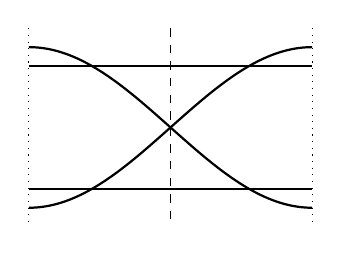
\begin{tikzpicture}[x=0.6cm,y=0.6cm]
  \draw[thick] (0,1.3) -- (6,1.3); % 管の上側の壁を表す直線
  \draw[thick] (0,-1.3) -- (6,-1.3); % 管の下側の壁を表す直線
  \draw[thick,domain=0:6,samples=60,smooth,variable=\x]
    plot ({\x},{1.7*cos(30*\x)}); % 変位の波形（上半分）。管の壁をはみ出すよう振幅を大きくしている
  \draw[thick,domain=0:6,samples=60,smooth,variable=\x]
    plot ({\x},{-1.7*cos(30*\x)}); % 変位の波形（下半分）。上側と対称な振動の様子を表す
  \draw[dashed] (3,2.1) -- (3,-2.1); % 中央にある節の位置を示す点線（波形・管の壁よりも長く伸ばしている）
  \draw[dotted] (0,2.1) -- (0,-2.1); % 左端（開口端）にある腹の位置を示す点線
  \draw[dotted] (6,2.1) -- (6,-2.1); % 右端（開口端）にある腹の位置を示す点線
\end{tikzpicture}}
& 基本振動 & $\lambda_1 = 2\ell = \dfrac{2\ell}{1}$ & $f_1 = \dfrac{1}{2\ell}V$ \\
\cline{2-4} % この行の下側の罫線

% ---- 2倍振動 (n=2) ----
\makebox[3.6cm][l]{\hspace{-1.2cm}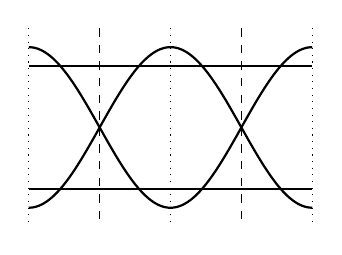
\begin{tikzpicture}[x=0.6cm,y=0.6cm]
  \draw[thick] (0,1.3) -- (6,1.3); % 管の上側の壁を表す直線
  \draw[thick] (0,-1.3) -- (6,-1.3); % 管の下側の壁を表す直線
  \draw[thick,domain=0:6,samples=60,smooth,variable=\x]
    plot ({\x},{1.7*cos(60*\x)}); % 変位の波形（上半分）。管の壁をはみ出す振幅
  \draw[thick,domain=0:6,samples=60,smooth,variable=\x]
    plot ({\x},{-1.7*cos(60*\x)}); % 変位の波形（下半分）
  \draw[dashed] (1.5,2.1) -- (1.5,-2.1); % 1つ目の節の位置を示す点線
  \draw[dashed] (4.5,2.1) -- (4.5,-2.1); % 2つ目の節の位置を示す点線
  \draw[dotted] (0,2.1) -- (0,-2.1); % 左端（開口端）にある腹の位置を示す点線
  \draw[dotted] (3,2.1) -- (3,-2.1); % 中央（内部）にある腹の位置を示す点線
  \draw[dotted] (6,2.1) -- (6,-2.1); % 右端（開口端）にある腹の位置を示す点線
\end{tikzpicture}}
& 2倍振動 & $\lambda_2 = \ell = \dfrac{2\ell}{2}$ & $f_2 = \dfrac{2}{2\ell}V$ \\
\cline{2-4}

% ---- 3倍振動 (n=3) ----
\makebox[3.6cm][l]{\hspace{-1.2cm}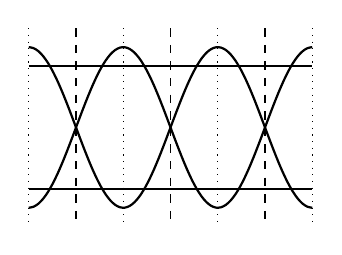
\begin{tikzpicture}[x=0.6cm,y=0.6cm]
  \draw[thick] (0,1.3) -- (6,1.3); % 管の上側の壁を表す直線
  \draw[thick] (0,-1.3) -- (6,-1.3); % 管の下側の壁を表す直線
  \draw[thick,domain=0:6,samples=60,smooth,variable=\x]
    plot ({\x},{1.7*cos(90*\x)}); % 変位の波形（上半分）
  \draw[thick,domain=0:6,samples=60,smooth,variable=\x]
    plot ({\x},{-1.7*cos(90*\x)}); % 変位の波形（下半分）
  \draw[dashed] (1,2.1) -- (1,-2.1); % 1つ目の節の位置を示す点線
  \draw[dashed] (3,2.1) -- (3,-2.1); % 2つ目の節の位置を示す点線
  \draw[dashed] (5,2.1) -- (5,-2.1); % 3つ目の節の位置を示す点線
  \draw[dotted] (0,2.1) -- (0,-2.1); % 左端（開口端）にある腹の位置を示す点線
  \draw[dotted] (2,2.1) -- (2,-2.1); % 1つ目の内部の腹の位置を示す点線
  \draw[dotted] (4,2.1) -- (4,-2.1); % 2つ目の内部の腹の位置を示す点線
  \draw[dotted] (6,2.1) -- (6,-2.1); % 右端（開口端）にある腹の位置を示す点線
\end{tikzpicture}}
& 3倍振動 & $\lambda_3 = \dfrac{2\ell}{3}$ & $f_3 = \dfrac{3}{2\ell}V$ \\
\cline{2-4}

% ---- n倍振動（両端に2ループずつ表示、中央は「…」で省略。節の点線は付けない） ----
\makebox[3.6cm][l]{\hspace{-1.2cm}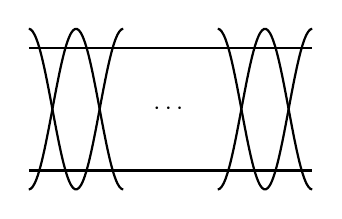
\begin{tikzpicture}[x=0.6cm,y=0.6cm]
  \draw[thick] (0,1.3) -- (6,1.3); % 管の上側の壁を表す直線（全体）
  \draw[thick] (0,-1.3) -- (6,-1.3); % 管の下側の壁を表す直線（全体）

  % 左端2ループ分の波形（上半分）。管の壁をはみ出す振幅にしている
  \draw[thick,domain=0:2,samples=50,smooth,variable=\x]
    plot ({\x},{1.7*cos(180*\x)});
  % 左端2ループ分の波形（下半分）
  \draw[thick,domain=0:2,samples=50,smooth,variable=\x]
    plot ({\x},{-1.7*cos(180*\x)});

  % 右端2ループ分の波形（上半分）。左端と対称なパターン
  \draw[thick,domain=4:6,samples=50,smooth,variable=\x]
    plot ({\x},{1.7*cos(180*\x)});
  % 右端2ループ分の波形（下半分）
  \draw[thick,domain=4:6,samples=50,smooth,variable=\x]
    plot ({\x},{-1.7*cos(180*\x)});

  \node[font=\small] at (3,0) {$\cdots$}; % 中央部分：波形を描かず、多数のループが続くことを省略記号で示す
\end{tikzpicture}}
& n倍振動 & $\lambda_n = \dfrac{2\ell}{n}$ & $f_n = \dfrac{n}{2\ell}V$ \\
\cline{2-4}
\end{tabular}
\end{center}

\clearpage
% -------------------------------------------------------------------
\subbanner{閉管の振動}
\begin{center}
\renewcommand{\arraystretch}{2.6}
\begin{tabular}{cc|c|c}
\cline{2-4} % 表部分（2〜4列目）の上側の罫線。気柱の図の列には引かない

% ---- ヘッダー行 ----
\makebox[3.6cm][l]{\hspace{-1.2cm}\begin{tikzpicture}[x=1cm,y=1cm]
  \draw[<->,>=stealth] (0,0) -- (3.6,0); % 気柱（管）全体の長さ l を示す両矢印
  \node[font=\small] at (1.8,0.35) {$\ell\,[\mathrm{m}]$}; % 矢印の上に長さのラベルを表示
\end{tikzpicture}}
& % 振動の名称列（ヘッダー行なので空欄）
& \textbf{波長 $\lambda\,[\mathrm{m}]$} % 波長列の見出し
& \textbf{振動数 $f\,[\mathrm{Hz}]$} \\ % 振動数列の見出し
\cline{2-4}

% ---- 基本振動 (m=1) ----
\makebox[3.6cm][l]{\hspace{-1.2cm}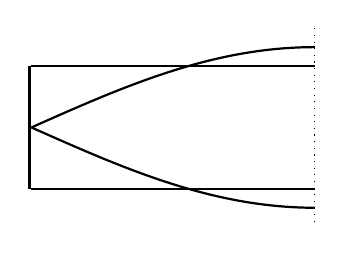
\begin{tikzpicture}[x=0.6cm,y=0.6cm]
  \fill[black] (-0.08,-1.3) rectangle (0,1.3); % 閉端（固定壁）を表す黒い長方形
  \draw[thick] (0,1.3) -- (6,1.3); % 管の上側の壁を表す直線
  \draw[thick] (0,-1.3) -- (6,-1.3); % 管の下側の壁を表す直線
  \draw[thick,domain=0:6,samples=60,smooth,variable=\x]
    plot ({\x},{1.7*sin(15*\x)}); % 変位の波形（上半分）。管の壁をはみ出すよう振幅を大きくしている
  \draw[thick,domain=0:6,samples=60,smooth,variable=\x]
    plot ({\x},{-1.7*sin(15*\x)}); % 変位の波形（下半分）
  \draw[dotted] (6,2.1) -- (6,-2.1); % 右端（開口端）にある腹の位置を示す点線
\end{tikzpicture}}
& 基本振動 & $\lambda_1 = 4\ell = \dfrac{4\ell}{1}$ & $f_1 = \dfrac{1}{4\ell}V$ \\
\cline{2-4}

% ---- 3倍振動 (m=3) ----
\makebox[3.6cm][l]{\hspace{-1.2cm}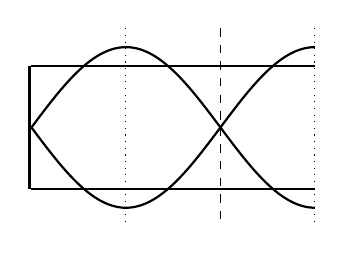
\begin{tikzpicture}[x=0.6cm,y=0.6cm]
  \fill[black] (-0.08,-1.3) rectangle (0,1.3); % 閉端（固定壁）を表す黒い長方形
  \draw[thick] (0,1.3) -- (6,1.3); % 管の上側の壁を表す直線
  \draw[thick] (0,-1.3) -- (6,-1.3); % 管の下側の壁を表す直線
  \draw[thick,domain=0:6,samples=60,smooth,variable=\x]
    plot ({\x},{1.7*sin(45*\x)}); % 変位の波形（上半分）。管の壁をはみ出す振幅
  \draw[thick,domain=0:6,samples=60,smooth,variable=\x]
    plot ({\x},{-1.7*sin(45*\x)}); % 変位の波形（下半分）
  \draw[dashed] (4,2.1) -- (4,-2.1); % 管内部にある節の位置を示す点線（波形・管の壁よりも長く伸ばしている）
  \draw[dotted] (2,2.1) -- (2,-2.1); % 内部にある腹の位置を示す点線
  \draw[dotted] (6,2.1) -- (6,-2.1); % 右端（開口端）にある腹の位置を示す点線
\end{tikzpicture}}
& 3倍振動 & $\lambda_3 = \dfrac{4\ell}{3}$ & $f_3 = \dfrac{3}{4\ell}V$ \\
\cline{2-4}

% ---- 5倍振動 (m=5) ----
\makebox[3.6cm][l]{\hspace{-1.2cm}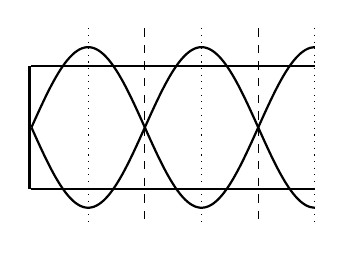
\begin{tikzpicture}[x=0.6cm,y=0.6cm]
  \fill[black] (-0.08,-1.3) rectangle (0,1.3); % 閉端（固定壁）を表す黒い長方形
  \draw[thick] (0,1.3) -- (6,1.3); % 管の上側の壁を表す直線
  \draw[thick] (0,-1.3) -- (6,-1.3); % 管の下側の壁を表す直線
  \draw[thick,domain=0:6,samples=60,smooth,variable=\x]
    plot ({\x},{1.7*sin(75*\x)}); % 変位の波形（上半分）
  \draw[thick,domain=0:6,samples=60,smooth,variable=\x]
    plot ({\x},{-1.7*sin(75*\x)}); % 変位の波形（下半分）
  \draw[dashed] (2.4,2.1) -- (2.4,-2.1); % 1つ目の節の位置を示す点線
  \draw[dashed] (4.8,2.1) -- (4.8,-2.1); % 2つ目の節の位置を示す点線
  \draw[dotted] (1.2,2.1) -- (1.2,-2.1); % 1つ目の内部の腹の位置を示す点線
  \draw[dotted] (3.6,2.1) -- (3.6,-2.1); % 2つ目の内部の腹の位置を示す点線
  \draw[dotted] (6,2.1) -- (6,-2.1); % 右端（開口端）にある腹の位置を示す点線
\end{tikzpicture}}
& 5倍振動 & $\lambda_5 = \dfrac{4\ell}{5}$ & $f_5 = \dfrac{5}{4\ell}V$ \\
\cline{2-4}

% ---- (2n-1)倍振動（両端に2ループずつ表示、中央は「…」で省略。節の点線は付けない） ----
\makebox[3.6cm][l]{\hspace{-1.2cm}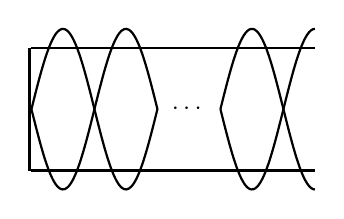
\begin{tikzpicture}[x=0.6cm,y=0.6cm]
  \fill[black] (-0.08,-1.3) rectangle (0,1.3); % 閉端（固定壁）を表す黒い長方形
  \draw[thick] (0,1.3) -- (6,1.3); % 管の上側の壁を表す直線（全体）
  \draw[thick] (0,-1.3) -- (6,-1.3); % 管の下側の壁を表す直線（全体）

  % 閉端側2ループ分の波形（上半分）。管の壁をはみ出す振幅にしている
  \draw[thick,domain=0:2.667,samples=50,smooth,variable=\x]
    plot ({\x},{1.7*sin(135*\x)});
  % 閉端側2ループ分の波形（下半分）
  \draw[thick,domain=0:2.667,samples=50,smooth,variable=\x]
    plot ({\x},{-1.7*sin(135*\x)});

  % 開端側2ループ分の波形（上半分）
  \draw[thick,domain=4:6,samples=50,smooth,variable=\x]
    plot ({\x},{1.7*sin(135*\x)});
  % 開端側2ループ分の波形（下半分）
  \draw[thick,domain=4:6,samples=50,smooth,variable=\x]
    plot ({\x},{-1.7*sin(135*\x)});

  \node[font=\small] at (3.333,0) {$\cdots$}; % 中央部分：波形を描かず、多数のループが続くことを省略記号で示す
\end{tikzpicture}}
& $(2n-1)$倍振動 & $\lambda_{2n-1} = \dfrac{4\ell}{2n-1}$ & $f_{2n-1} = \dfrac{2n-1}{4\ell}V$ \\
\cline{2-4}
\end{tabular}
\end{center}

閉管の境界条件より，閉口端は\textbf{必ず節}になるため，共鳴できる振動数は基本振動数の\textbf{奇数倍}に限られる。
% ------------------------------------------------------
\subbanner{開口端補正}

開口において、実際には定在波の腹は管口の少し\textbf{外側}にできる。このずれを\textbf{開口端補正}という。
同じ管では，振動数によらず開口端補正 $\Delta x$ はほぼ一定の値になる。

\begin{center}
  \begin{tikzpicture}[x=1.1cm,y=1.1cm]
  \def\Lphys{5.4} % 開口端(実際の管の端)の位置：3倍振動の場合と同じ長さ
  \def\Ltrue{6}   % 真の腹の位置(開口端補正 \Delta x は管の形状で決まるので同じ値)
  \draw[very thick] (0,-0.4) -- (0,0.4); % 閉端(壁)
  \draw[thick] (0,0.4) -- (\Lphys,0.4); % 管の上側の壁
  \draw[thick] (0,-0.4) -- (\Lphys,-0.4); % 管の下側の壁
  \draw[thick,domain=0:\Lphys,samples=100] plot (\x,{0.55*sin(90*\x/\Ltrue)}); % 管内の定在波(上)：1ループのみ
  \draw[thick,domain=0:\Lphys,samples=100] plot (\x,{-0.55*sin(90*\x/\Ltrue)}); % 管内の定在波(下)
  \draw[thick,domain=\Lphys:\Ltrue,samples=20] plot (\x,{0.55*sin(90*\x/\Ltrue)}); % 開口端より外側，真の腹まで(上)：実際に存在する波なので実線
  \draw[thick,domain=\Lphys:\Ltrue,samples=20] plot (\x,{-0.55*sin(90*\x/\Ltrue)}); % 開口端より外側，真の腹まで(下)
  \draw[dashed] (0,0.8) -- (0,-1.4); \node[above,font=\scriptsize] at (0,0.85) {節};
  \draw[dashed] (\Ltrue,0.8) -- (\Ltrue,-1.4); \node[above,font=\scriptsize] at (\Ltrue,0.85) {腹};
  \draw[dashed] (\Lphys,0.7) -- (\Lphys,-0.7); % 開口端(実際の管の端)の位置を示す線
  \draw[<->] (\Lphys,-0.65) -- (\Ltrue,-0.65) node[midway,below,font=\scriptsize]{$\Delta x$};
  \draw[<->] (0,-1.2) -- (\Ltrue,-1.2) node[midway,below,font=\scriptsize]{$\dfrac{\lambda}{4}$};
  \node[below,font=\scriptsize] at (0.15,-0.55) {閉};
\end{tikzpicture}
\end{center}
\begin{center}
\begin{tikzpicture}[x=1.1cm,y=1.1cm]
  \def\Lphys{5.4} % 開口端(実際の管の端)の位置
  \def\Ltrue{6}   % 真の腹(2つ目の節から\lambda/4進んだ位置)
  \draw[very thick] (0,-0.4) -- (0,0.4); % 閉端(壁)
  \draw[thick] (0,0.4) -- (\Lphys,0.4); % 管の上側の壁(閉端〜開口端)
  \draw[thick] (0,-0.4) -- (\Lphys,-0.4); % 管の下側の壁
  \draw[thick,domain=0:\Lphys,samples=100] plot (\x,{0.55*sin(45*\x)}); % 管内にある定在波(上)：1つ目のループはそのまま，2つ目は開口端で切れる
  \draw[thick,domain=0:\Lphys,samples=100] plot (\x,{-0.55*sin(45*\x)}); % 管内にある定在波(下)
  \draw[thick,domain=\Lphys:\Ltrue,samples=20] plot (\x,{0.55*sin(45*\x)}); % 開口端より外側，真の腹まで(上)：実際に存在する波なので実線
  \draw[thick,domain=\Lphys:\Ltrue,samples=20] plot (\x,{-0.55*sin(45*\x)}); % 開口端より外側，真の腹まで(下)
  \draw[dashed] (0,0.8) -- (0,-1.4); \node[above,font=\scriptsize] at (0,0.85) {節};
  \draw[dashed] (2,0.8) -- (2,-1.4); \node[above,font=\scriptsize] at (2,0.85) {腹};
  \draw[dashed] (4,0.8) -- (4,-1.4); \node[above,font=\scriptsize] at (4,0.85) {節};
  \draw[dashed] (\Ltrue,0.8) -- (\Ltrue,-1.4); \node[above,font=\scriptsize] at (\Ltrue,0.85) {腹};
  \draw[dashed] (\Lphys,0.7) -- (\Lphys,-0.7); % 開口端(実際の管の端)の位置を示す線
  \draw[<->] (\Lphys,-0.65) -- (\Ltrue,-0.65) node[midway,below,font=\scriptsize]{$\Delta x$};
  \draw[<->] (4,-1.2) -- (\Ltrue,-1.2) node[midway,below,font=\scriptsize]{$\dfrac{\lambda}{4}$};
  \node[below,font=\scriptsize] at (0.15,-0.55) {閉};
\end{tikzpicture}
\end{center}

\clearpage
% ========================================================================
\banner{n倍振動の振動数・音速を求める手順}

弦や気柱の固有振動の問題は，次の3ステップで機械的に解くことができる。

\subbanner{STEP1：定在波を図示する}

\textbf{(1)境界条件を確認する}\quad 端の種類によって，そこが定在波の節になるか腹になるかが決まる。

\begin{formulabox}
\begin{center}
\begin{tabular}{@{}lccl@{}}
\toprule
 & 端① & 他端② & 両端の関係 \\
\midrule
弦 & 固定端 & 固定端 & 節 -- 節 \\
開管 & 自由端 & 自由端 & 腹 -- 腹 \\
閉管 & 固定端 & 自由端 & 節 -- 腹 \\
\bottomrule
\end{tabular}
\end{center}
\end{formulabox}

\begin{pointbox}
\textbf{反射の考え方}：\\
閉じている端(壁・水面など動けない境界)では\textbf{固定端反射}が起こる→媒質が動けないので\textbf{節}になる。\\
開いている端(自由に動ける境界)では\textbf{自由端反射}が起こり\textbf{腹}になる。
\end{pointbox}

\textbf{(2)基本振動($n=1$)から順に作図する}\quad 境界条件を満たしたまま，節・腹を1つずつ増やして倍振動を作図していく。



\subbanner{STEP2：装置の長さ $L$ と波長 $\lambda$ を対応させる}

図に節・腹がいくつ現れるかを数えると，$\lambda/4$を単位として$L$を表すことができる。
\begin{formulabox}
\begin{center}
\textbf{$L$と$\lambda$の関係}\\[4pt]
$\boxed{\,L = \bigcirc \times \dfrac{\lambda}{4}\,}\qquad\Longleftrightarrow\qquad \boxed{\,\lambda = \dfrac{4L}{\bigcirc}\,}$\\[4pt]
{\footnotesize $\bigcirc$：図から読み取った$\lambda/4$の個数}
\end{center}
\end{formulabox}

\noindent
\begin{minipage}[t]{0.48\textwidth}
\centering
{\small\textbf{例1：開管の基本振動}}\\[4pt]
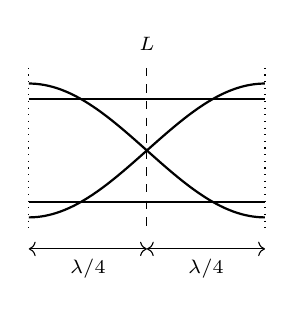
\begin{tikzpicture}[x=0.5cm,y=0.5cm]
  \draw[thick] (0,1.3) -- (6,1.3); \draw[thick] (0,-1.3) -- (6,-1.3);
  \draw[thick,domain=0:6,samples=60,smooth,variable=\x] plot ({\x},{1.7*cos(30*\x)});
  \draw[thick,domain=0:6,samples=60,smooth,variable=\x] plot ({\x},{-1.7*cos(30*\x)});
  \draw[dashed] (3,2.1) -- (3,-2.1);
  \draw[dotted] (0,2.1) -- (0,-2.1); \draw[dotted] (6,2.1) -- (6,-2.1);
  \draw[<->] (0,-2.5) -- (3,-2.5) node[midway,below,font=\scriptsize]{$\lambda/4$};
  \draw[<->] (3,-2.5) -- (6,-2.5) node[midway,below,font=\scriptsize]{$\lambda/4$};
  \node[above,font=\scriptsize] at (3,2.3) {$L$};
\end{tikzpicture}\\[4pt]
{\footnotesize 両端が腹 $\to$ $\lambda/4$が2個分}
\[
L=2\times\frac{\lambda}{4} \ \Longrightarrow\ \bigcirc=2 \ \Longrightarrow\ \lambda=\frac{4L}{2}=2L
\]
\end{minipage}\hfill
\begin{minipage}[t]{0.48\textwidth}
\centering
{\small\textbf{例2：閉管の基本振動}}\\[4pt]
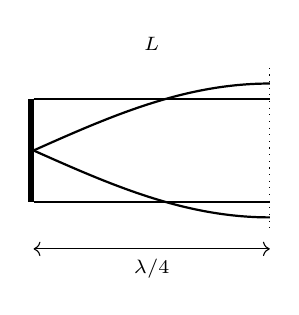
\begin{tikzpicture}[x=0.5cm,y=0.5cm]
  \fill[black] (-0.15,-1.3) rectangle (0,1.3);
  \draw[thick] (0,1.3) -- (6,1.3); \draw[thick] (0,-1.3) -- (6,-1.3);
  \draw[thick,domain=0:6,samples=60,smooth,variable=\x] plot ({\x},{1.7*sin(15*\x)});
  \draw[thick,domain=0:6,samples=60,smooth,variable=\x] plot ({\x},{-1.7*sin(15*\x)});
  \draw[dotted] (6,2.1) -- (6,-2.1);
  \draw[<->] (0,-2.5) -- (6,-2.5) node[midway,below,font=\scriptsize]{$\lambda/4$};
  \node[above,font=\scriptsize] at (3,2.3) {$L$};
\end{tikzpicture}\\[4pt]
{\footnotesize 節(閉端)から腹(開端)まで $\to$ $\lambda/4$が1個分}
\[
L=1\times\frac{\lambda}{4} \ \Longrightarrow\ \bigcirc=1 \ \Longrightarrow\ \lambda=\frac{4L}{1}=4L
\]
\end{minipage}

\begin{pointbox}
同じ長さ$L$の管でも，開管($\lambda=2L$)と閉管($\lambda=4L$)では波長が異なる。これは，境界条件によって$\lambda/4$が何個分入るか($\bigcirc$の値)が変わるためである。
\end{pointbox}
\clearpage
\subbanner{STEP3：$v=f\lambda$ を使って残りの物理量を求める}

$v=f\lambda$は波の種類によらず常に成り立つ。$f$，$\lambda$，$v$のうち2つが分かれば，残り1つが求まる。STEP2で$\lambda$は求まっているので，あとは$f$と$v$のどちらか一方を，波の種類ごとの別の式から求める。

\begin{formulabox}
\begin{center}
\textbf{弦の場合}\\[4pt]
張力$S$，線密度$\rho$が分かっている$\Rightarrow$ $\boxed{\,v=\sqrt{\dfrac{S}{\rho}}\,}$ で $v$ を求め，$f=\dfrac{v}{\lambda}$\\[6pt]
振動数$f$が分かっている$\Rightarrow$ $\boxed{\,v=f\lambda\,}$ で $v$ を求める
\end{center}
\end{formulabox}

\begin{formulabox}
\begin{center}
\textbf{気柱の場合}\\[4pt]
気温$t$が分かっている$\Rightarrow$ $\boxed{\,V=331.5+0.6t\,}$ で $V$ を求め，$f=\dfrac{V}{\lambda}$\\[6pt]
振動数$f$が分かっている$\Rightarrow$ $\boxed{\,V=f\lambda\,}$ で $V$ を求める
\end{center}
\end{formulabox}



\begin{pointbox}
弦と開管は，どちらも「両端が同じ種類」という境界条件が同じため，$L$と$\lambda$の関係も同じ形($L=n\lambda/2$)になる。閉管だけは境界条件が異なるため，別の形($L=n\lambda/4$，$n$は奇数)になる。
\end{pointbox}


\clearpage



\begin{comment}

試験管の口に息を吹き込むと音が鳴る。水を入れる量(気柱の長さ)を変えると，音の高さが変わる。

\begin{center}
\begin{tikzpicture}[x=1cm,y=1cm]
  % 短い気柱(上)：高い音
  \begin{scope}[yshift=4.2cm]
    \draw[thick] (0,0) rectangle (1.3,3.0);
    \fill[black!15] (0,0) rectangle (1.3,2.0);
    \draw[-{Latex[length=2.5mm]}] (0.65,3.6) -- (0.65,3.05);
    \node[above,font=\scriptsize] at (0.65,3.7) {息};
    \draw[<->] (1.7,2.0) -- (1.7,3.0) node[midway,right,font=\scriptsize]{気柱(短い)};
    \node[right,font=\scriptsize] at (2.8,1.0) {高い音($f$ 大)};
  \end{scope}
  % 長い気柱(下)：低い音
  \begin{scope}[yshift=0cm]
    \draw[thick] (0,0) rectangle (1.3,3.0);
    \fill[black!15] (0,0) rectangle (1.3,0.6);
    \draw[-{Latex[length=2.5mm]}] (0.65,3.6) -- (0.65,3.05);
    \node[above,font=\scriptsize] at (0.65,3.7) {息};
    \draw[<->] (1.7,0.6) -- (1.7,3.0) node[midway,right,font=\scriptsize]{気柱(長い)};
    \node[right,font=\scriptsize] at (2.8,1.6) {低い音($f$ 小)};
  \end{scope}
\end{tikzpicture}
\end{center}

\begin{pointbox}
気柱が短いほど固有振動数は大きく，音は高くなる(閉管：$f_1=V/4L$，$L\downarrow \Rightarrow f_1\uparrow$)。
\end{pointbox}

\clearpage


\subbanner{実験：閉管の共鳴(水面を下げる)}

おんさを管口に近づけ，水面を徐々に下げていくと，気柱の長さが特定の値になったときに共鳴して音が大きく聞こえる。

\begin{center}
\begin{tikzpicture}[x=1cm,y=1cm]
  \draw[thick] (1.0,6.4) -- (1.0,7.4); \draw[thick] (1.6,6.4)--(1.6,7.4);
  \draw[thick] (1.0,6.4) arc (180:360:0.3);
  \node[above,font=\scriptsize] at (1.3,7.5) {おんさ(振動数 $f$)};
  \draw[thick] (0,0) -- (0,6.2); \draw[thick] (1.2,0) -- (1.2,6.2);
  \fill[black!15] (0,0) rectangle (1.2,2.0);
  \node[right,font=\scriptsize] at (1.3,1.0) {水};
  \draw[<->] (1.9,2.0) -- (1.9,6.2) node[midway,right,font=\scriptsize]{気柱の長さ};
  \node[below,font=\scriptsize] at (0.6,-0.3){ガラス円筒};
  \draw[thick] (1.2,0.3) .. controls (2.6,0.3) and (2.6,1.2) .. (3.4,1.2);
  \draw[thick] (3.2,0.8) rectangle (4.2,2.4);
  \fill[black!15] (3.2,0.8) rectangle (4.2,2.0); % ガラス円筒側の水面(y=2.0)と高さを揃える
  \node[below,font=\scriptsize] at (3.7,0.6){水だめ(上下させ水位調整)};
\end{tikzpicture}
\end{center}

\begin{center}
\begin{tabular}{@{}ccc@{}}
\toprule
測定回数 & $L_1$[cm](第1共鳴点) & $L_2$[cm](第2共鳴点) \\
\midrule
1 & 18.4 & 56.9 \\
2 & 18.7 & 57.1 \\
3 & 18.7 & 57.3 \\
\midrule
平均 & 18.6 & 57.1 \\
\bottomrule
\end{tabular}
\end{center}
\begin{center}
{\footnotesize 気温\SI{17.1}{\celsius}，標準おんさの振動数\SI{440}{Hz}，$L_2-L_1=\SI{38.5}{cm}$}
\end{center}

\clearpage
\begin{center}
\begin{tikzpicture}[x=1cm,y=1cm]
  \begin{scope}[yshift=0cm]
    \def\L{2.0}
    \draw[very thick] (0,-0.4) -- (0,0.4);
    \draw[thick] (0,0.4) -- (\L,0.4); \draw[thick] (0,-0.4) -- (\L,-0.4);
    \draw[thick,domain=0:\L,samples=80] plot (\x,{0.5*sin(1*90*\x/\L)});
    \draw[thick,dashed,domain=0:\L,samples=80] plot (\x,{-0.5*sin(1*90*\x/\L)});
    \fill (0,0) circle (1.3pt);
    \node[right,font=\scriptsize] at (\L+0.2,0) {第1共鳴点：$L_1=\SI{18.6}{cm}$(基本振動)};
    \node[below,font=\scriptsize] at (0.15,-0.55) {水面};
  \end{scope}
  \begin{scope}[yshift=-2.2cm]
    \def\L{6.0}
    \draw[very thick] (0,-0.4) -- (0,0.4);
    \draw[thick] (0,0.4) -- (\L,0.4); \draw[thick] (0,-0.4) -- (\L,-0.4);
    \draw[thick,domain=0:\L,samples=50] plot (\x,{0.5*sin(3*90*\x/\L)});
    \draw[thick,dashed,domain=0:\L,samples=50] plot (\x,{-0.5*sin(3*90*\x/\L)});
    \fill (0,0) circle (1.3pt);
    \node[right,font=\scriptsize] at (\L+0.2,0) {第2共鳴点：$L_2=\SI{57.1}{cm}$(3倍振動)};
    \node[below,font=\scriptsize] at (0.15,-0.55) {水面};
  \end{scope}
\end{tikzpicture}
\end{center}

図より，$L_2-L_1$ は定在波の半波長に等しい。

\[
L_2-L_1=\frac{\lambda}{2} \quad\Rightarrow\quad \lambda=2\times\SI{38.5}{cm}=\SI{77.0}{cm}
\]

\begin{pointbox}
気温\SI{17.1}{\celsius}のときの理論値は $V=331.5+0.6\times17.1\approx\SI{341.8}{m/s}$，$\lambda=V/f=341.8/440\approx\SI{77.7}{cm}$。実験値 \SI{77.0}{cm} とよく一致する。
\end{pointbox}

\clearpage

\subbanner{実験：開管の共鳴(振動数を変える)}

長さ一定の開管に対し，スピーカーの振動数を0からゆっくり増していくと，複数の振動数で共鳴が起こる。

\begin{center}
\begin{tikzpicture}[x=1cm,y=1cm]
  \draw[thick] (0,1.4) -- (6,1.4); \draw[thick] (0,0) -- (6,0); % 開管：上下の壁のみ(両端は開いているので縦線は引かない)
  \node[below,font=\scriptsize] at (3,-0.3){開管(長さ一定)};
  \draw[thick,fill=black!10] (-1.1,0.2) rectangle (0,1.2);
  \node[below,font=\scriptsize] at (-0.55,0.05){スピーカー};
  \draw[thick] (-2.4,0.5) rectangle (-1.3,1.3);
  \node[above,font=\scriptsize] at (-1.85,1.35){発振器};
  \draw[-{Latex[length=2.5mm]}] (-1.3,0.9)--(-1.15,0.9);
  \node[right,font=\scriptsize] at (6.1,0.7){振動数を上げていく};
\end{tikzpicture}
\end{center}

\begin{center}
\begin{tabular}{@{}cccc@{}}
\toprule
測定回数 & $f_1$[Hz] & $f_2$[Hz] & $f_3$[Hz] \\
\midrule
1 & 485 & 980 & 1450 \\
2 & 490 & 970 & 1465 \\
3 & 490 & 980 & 1470 \\
\midrule
平均 & 488 & 977 & 1462 \\
$f_n/f_1$ & 1 & 2.00 & 3.00 \\
\bottomrule
\end{tabular}
\end{center}

\clearpage
\begin{center}
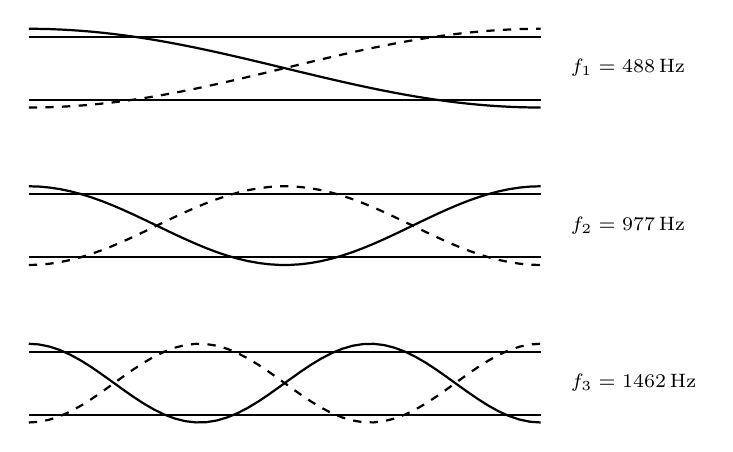
\begin{tikzpicture}[x=1.3cm,y=1cm]
  \def\L{5}
  \foreach \n/\freqlab/\yoff in {1/{488}/0, 2/{977}/-2.0, 3/{1462}/-4.0}{
    \begin{scope}[yshift=\yoff cm]
      \draw[thick] (0,0.4) -- (\L,0.4); \draw[thick] (0,-0.4) -- (\L,-0.4);
      \draw[thick,domain=0:\L,samples=50] plot (\x,{0.5*cos(\n*180*\x/\L)});
      \draw[thick,dashed,domain=0:\L,samples=50] plot (\x,{-0.5*cos(\n*180*\x/\L)});
      \node[right,font=\scriptsize] at (\L+0.2,0) {$f_{\n}=\SI{\freqlab}{Hz}$};
    \end{scope}
  }
\end{tikzpicture}
\end{center}

$f_2,f_3$ は $f_1$ のほぼ2倍，3倍になっている(整数倍の関係)。



\clearpage




\clearpage
\subbanner{参考：管口での反射(パルス波)}

\begin{center}
\begin{tikzpicture}[x=1cm,y=1cm]
  % 閉端(上)
  \begin{scope}[yshift=2.4cm]
    \draw[thick] (0,0) -- (5,0);
    \draw[very thick] (5,-0.5) -- (5,0.5);
    \draw[thick,domain=1:2.4,samples=40] plot(\x,{0.5*sin(180*(\x-1)/1.4)});
    \node[above,font=\scriptsize] at (1.7,0.6) {入射パルス};
    \draw[thick,dashed,domain=3.6:5,samples=40] plot(\x,{-0.5*sin(180*(\x-3.6)/1.4)});
    \node[below,font=\scriptsize] at (4.3,-0.7) {反射パルス(山→谷)};
    \node[below,font=\scriptsize] at (5,-1.1){閉端＝固定端反射};
  \end{scope}
  % 開端(下)
  \begin{scope}[yshift=0cm]
    \draw[thick] (0,0) -- (5,0);
    \draw[thick,domain=1:2.4,samples=40] plot(\x,{0.5*sin(180*(\x-1)/1.4)});
    \node[above,font=\scriptsize] at (1.7,0.6) {入射パルス};
    \draw[thick,dashed,domain=3.6:5,samples=40] plot(\x,{0.5*sin(180*(\x-3.6)/1.4)});
    \node[above,font=\scriptsize] at (4.3,0.6) {反射パルス(山→山)};
    \node[below,font=\scriptsize] at (5,-0.4){開端＝自由端反射};
  \end{scope}
\end{tikzpicture}
\end{center}

\begin{pointbox}
気柱内の音波の反射は，弦の反射と同じ考え方ができる。\\
\textbf{閉端}(変位0の条件) $\to$ \textbf{固定端反射}(山が谷になって返る)\\
\textbf{開端}(変位最大の条件) $\to$ \textbf{自由端反射}(山は山のまま返る)
\end{pointbox}

\clearpage
\subbanner{例題：気柱共鳴の測定}

\begin{examplebox}
振動数\SI{550}{Hz}のスピーカーの下でガラス管の水面を下げていくと，管口から\SI{13.5}{cm}と\SI{43.5}{cm}の位置で共鳴が起こった(閉管とみなせる)。
\begin{enumerate}[label=(\arabic*),itemsep=1pt]
  \item 音の波長を求めよ。
  \item 音速を求めよ。
  \item 開口端補正を求めよ。
\end{enumerate}
\end{examplebox}

\begin{center}
\begin{tikzpicture}[x=1cm,y=1cm]
  \begin{scope}[yshift=0cm]
    \draw[thick] (0,0) rectangle (1.6,4.5);
    \draw[fill=black!10] (0,0) rectangle (1.6,3.3);
    \node[right,font=\scriptsize] at (1.7,3.9) {水面(1回目)};
    \draw[<->] (2.4,3.3) -- (2.4,4.5) node[midway,right,font=\scriptsize] {$\SI{13.5}{cm}$};
  \end{scope}
  \begin{scope}[yshift=-5.6cm]
    \draw[thick] (0,0) rectangle (1.6,4.5);
    \draw[fill=black!10] (0,0) rectangle (1.6,1.0);
    \node[right,font=\scriptsize] at (1.7,0.5) {水面(2回目)};
    \draw[<->] (2.4,1.0) -- (2.4,4.5) node[midway,right,font=\scriptsize] {$\SI{43.5}{cm}$};
  \end{scope}
\end{tikzpicture}
\end{center}

\textbf{考え方}：2つの共鳴点の間隔は，定在波の\textbf{半波長}に等しい。

\[
\underbrace{43.5-13.5}_{\lambda/2}=\SI{30.0}{cm}
\quad\Rightarrow\quad
\lambda = \SI{60.0}{cm}
\]
\[
V=f\lambda = \SI{550}{Hz}\times\SI{0.600}{m}=\SI{330}{m/s}
\]
\[
\frac{\lambda}{4}=\SI{15.0}{cm},\qquad
\Delta x = 15.0-13.5=\SI{1.5}{cm}
\]

\begin{pointbox}
\textbf{解答}：(1) $\lambda=\SI{60.0}{cm}$\quad(2) $V=\SI{330}{m/s}$\quad(3) $\Delta x=\SI{1.5}{cm}$
\end{pointbox}

\clearpage

\begin{comment}
% ========================================================================
\banner{5. 波の式の導出 ―― $y$-$x$グラフから進行波の式へ}

\begin{center}
\begin{tikzpicture}[node distance=7mm]
\tikzset{flow/.style={draw,thick,rounded corners,fill=black!4,align=center,minimum width=6.6cm,minimum height=8mm,font=\small}}
\node[flow] (a) {波形を見る};
\node[flow,below=of a] (b) {波長・周期を理解する};
\node[flow,below=of b] (c) {位相を考える};
\node[flow,below=of c] (d) {波数・角周波数を定義する};
\node[flow,below=of d] (e) {波の式を導く};
\draw[-{Latex}] (a)--(b); \draw[-{Latex}] (b)--(c); \draw[-{Latex}] (c)--(d); \draw[-{Latex}] (d)--(e);
\end{tikzpicture}
\end{center}

\begin{cautionbox}
\boxed{\text{方針}}\quad この章では，$\boxed{y(x,t)=A\sin(kx-\omega t+\varphi)}$ を公式として\textbf{与えません}。$y$-$x$グラフと$y$-$t$グラフから出発し，最後に自分の手でこの式を導きます。
\end{cautionbox}

\clearpage
\subbanner{図1：$y$-$x$グラフ ―― ある時刻の波形}

「ある時刻において，波が空間的にどのような形をしているか」を表すグラフ。

\begin{center}
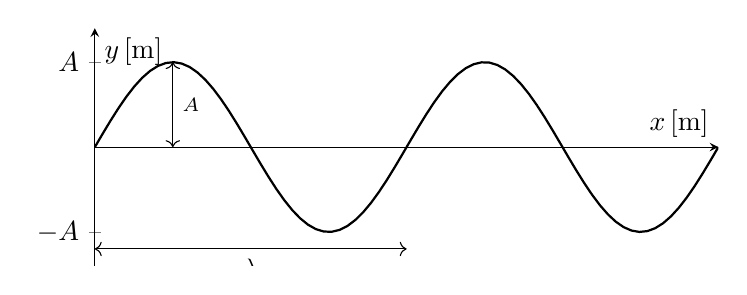
\begin{tikzpicture}
\begin{axis}[
  width=9.5cm,height=4.6cm,
  xlabel={$x\,[\si{m}]$}, ylabel={$y\,[\si{m}]$},
  axis lines=middle, xtick=\empty, ytick={-1,1},
  yticklabels={$-A$,$A$},
  xmin=0,xmax=2,ymin=-1.4,ymax=1.4,
  domain=0:2,samples=80,
]
\addplot[thick] {sin(360*x/1)};
\draw[<->] (axis cs:0,-1.2) -- (axis cs:1,-1.2) node[midway,below,font=\scriptsize]{$\lambda$};
\draw[<->] (axis cs:0.25,0) -- (axis cs:0.25,1) node[midway,right,font=\scriptsize]{$A$};
\end{axis}
\end{tikzpicture}
\end{center}

\begin{defbox}
$y$-$x$グラフから読み取れる量：$\boxed{\lambda=\text{波長}}$(波形が1回繰り返す長さ)
\end{defbox}

\subbanner{図2：$y$-$t$グラフ ―― ある位置の振動}

「ある位置において，媒質が時間的にどのように振動しているか」を表すグラフ。

\begin{center}
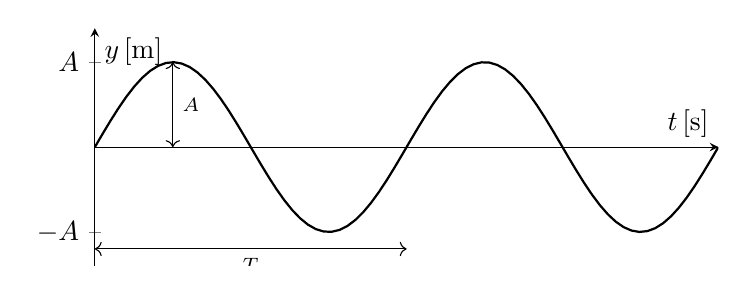
\begin{tikzpicture}
\begin{axis}[
  width=9.5cm,height=4.6cm,
  xlabel={$t\,[\si{s}]$}, ylabel={$y\,[\si{m}]$},
  axis lines=middle, xtick=\empty, ytick={-1,1},
  yticklabels={$-A$,$A$},
  xmin=0,xmax=2,ymin=-1.4,ymax=1.4,
  domain=0:2,samples=80,
]
\addplot[thick] {sin(360*x/1)};
\draw[<->] (axis cs:0,-1.2) -- (axis cs:1,-1.2) node[midway,below,font=\scriptsize]{$T$};
\draw[<->] (axis cs:0.25,0) -- (axis cs:0.25,1) node[midway,right,font=\scriptsize]{$A$};
\end{axis}
\end{tikzpicture}
\end{center}

\begin{defbox}
$y$-$t$グラフから読み取れる量：$\boxed{T=\text{周期}}$(同じ状態に戻るまでの時間)
\end{defbox}

\[
\boxed{f=\frac{1}{T}}
\]
\Meaning{周期 $T$ の逆数が，1秒あたりに振動する回数(振動数) $f$}

\clearpage
\subbanner{図3：$y$-$x$と$y$-$t$の違い}

この2つのグラフは非常に混同しやすい。必ず区別すること。

\begin{center}
\begin{tikzpicture}
\begin{groupplot}[
  group style={group size=1 by 2, vertical sep=1.3cm},
  width=9.5cm,height=3.4cm,
  axis lines=middle, xtick=\empty, ytick=\empty,
  ymin=-1.3,ymax=1.3, xmin=0,xmax=2,
  domain=0:2,samples=60,
  title style={font=\footnotesize},
]
\nextgroupplot[title={$y$-$x$：時刻 $t$ を固定して空間を見る},xlabel={$x$}]
\addplot[thick]{sin(360*x)};
\nextgroupplot[title={$y$-$t$：位置 $x$ を固定して時間を見る},xlabel={$t$}]
\addplot[thick]{sin(360*x)};
\end{groupplot}
\end{tikzpicture}
\end{center}

\begin{center}
\begin{tabular}{@{}lcc@{}}
\toprule
 & $y$-$x$ グラフ & $y$-$t$ グラフ \\
\midrule
固定するもの & 時刻 $t$ & 位置 $x$ \\
横軸 & $x$ & $t$ \\
表しているもの & 空間的な波形 & 1点の時間変化 \\
読み取る量 & 波長 $\lambda$ & 周期 $T$ \\
関係する量 & $k$ & $\omega$ \\
\bottomrule
\end{tabular}
\end{center}

\clearpage
\subbanner{図5：$y$-$x$グラフから波数 $k$ を導く}

時刻 $t=0$ の波形 $y(x,0)=A\sin(kx+\varphi)$ を考える。正弦波は1波長 $\lambda$ 進むと同じ状態に戻る。

\begin{center}
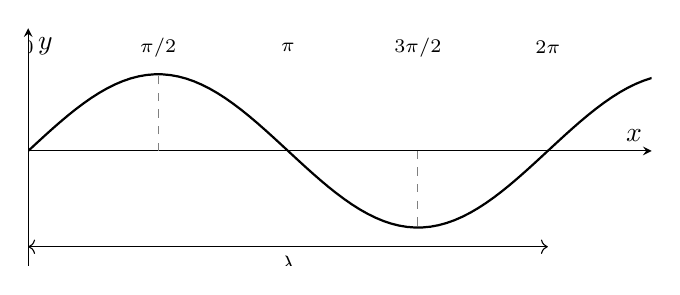
\begin{tikzpicture}
\begin{axis}[
  width=9.5cm,height=4.6cm,
  xlabel={$x$}, ylabel={$y$},
  axis lines=middle, xtick=\empty, ytick=\empty,
  xmin=0,xmax=1.2,ymin=-1.5,ymax=1.6,
  domain=0:1.2,samples=80,
]
\addplot[thick]{sin(360*x)};
\draw[<->] (axis cs:0,-1.25) -- (axis cs:1,-1.25) node[midway,below,font=\scriptsize]{$\lambda$};
\node[font=\scriptsize] at (axis cs:0,1.35) {$0$};
\node[font=\scriptsize] at (axis cs:0.25,1.35) {$\pi/2$};
\node[font=\scriptsize] at (axis cs:0.5,1.35) {$\pi$};
\node[font=\scriptsize] at (axis cs:0.75,1.35) {$3\pi/2$};
\node[font=\scriptsize] at (axis cs:1,1.35) {$2\pi$};
\draw[dashed,gray] (axis cs:0.25,0) -- (axis cs:0.25,1);
\draw[dashed,gray] (axis cs:0.75,0) -- (axis cs:0.75,-1);
\end{axis}
\end{tikzpicture}
\end{center}

つまり，1波長 $\lambda$ 進むごとに位相は $2\pi$ だけ変化する。

\[
k\lambda=2\pi
\]

\begin{formulabox}
\begin{center}
$\boxed{\,k=\dfrac{2\pi}{\lambda}\,}$
\end{center}
\end{formulabox}

\begin{defbox}
波数 $k$ は「単位長さあたりに位相がどれだけ変化するか」を表す量。単位は $\si{rad/m}$。
\end{defbox}

\Meaning{$\lambda\downarrow \ \Rightarrow\ k\uparrow$ ―― 波長が短いほど，単位長さあたりの位相変化が大きい}

\clearpage
\subbanner{図6：$y$-$t$グラフから角周波数 $\omega$ を導く}

位置 $x=x_0$ を固定して時間変化を見る。1周期 $T$ で位相は $2\pi$ 変化する。

\begin{center}
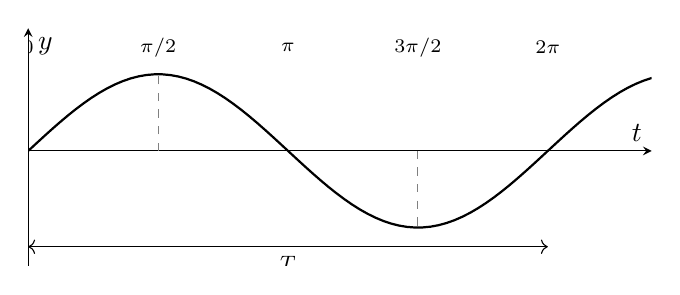
\begin{tikzpicture}
\begin{axis}[
  width=9.5cm,height=4.6cm,
  xlabel={$t$}, ylabel={$y$},
  axis lines=middle, xtick=\empty, ytick=\empty,
  xmin=0,xmax=1.2,ymin=-1.5,ymax=1.6,
  domain=0:1.2,samples=80,
]
\addplot[thick]{sin(360*x)};
\draw[<->] (axis cs:0,-1.25) -- (axis cs:1,-1.25) node[midway,below,font=\scriptsize]{$T$};
\node[font=\scriptsize] at (axis cs:0,1.35) {$0$};
\node[font=\scriptsize] at (axis cs:0.25,1.35) {$\pi/2$};
\node[font=\scriptsize] at (axis cs:0.5,1.35) {$\pi$};
\node[font=\scriptsize] at (axis cs:0.75,1.35) {$3\pi/2$};
\node[font=\scriptsize] at (axis cs:1,1.35) {$2\pi$};
\draw[dashed,gray] (axis cs:0.25,0) -- (axis cs:0.25,1);
\draw[dashed,gray] (axis cs:0.75,0) -- (axis cs:0.75,-1);
\end{axis}
\end{tikzpicture}
\end{center}

\[
\omega T=2\pi
\]

\begin{formulabox}
\begin{center}
$\boxed{\,\omega=\dfrac{2\pi}{T}\,}$
\end{center}
\end{formulabox}

$f=1/T$ より，

\[
\boxed{\,\omega=2\pi f\,}
\]

\begin{defbox}
角周波数 $\omega$ は「1秒間に位相が何 $\si{rad}$ 変化するか」を表す量。単位は $\si{rad/s}$。
\end{defbox}

\clearpage
\subbanner{対応関係のまとめ}

\begin{formulabox}
\begin{center}
$\boxed{\,y\text{-}x \ \Rightarrow\ \lambda \ \Rightarrow\ k=\dfrac{2\pi}{\lambda}\,}$
\end{center}
\end{formulabox}
\begin{formulabox}
\begin{center}
$\boxed{\,y\text{-}t \ \Rightarrow\ T \ \Rightarrow\ \omega=\dfrac{2\pi}{T}=2\pi f\,}$
\end{center}
\end{formulabox}

\[
\boxed{\text{空間方向の変化}\ \to\ k}
\qquad\qquad
\boxed{\text{時間方向の変化}\ \to\ \omega}
\]

\subbanner{波の速さ $v=f\lambda=\lambda/T$}

波は1周期 $T$ の間に1波長 $\lambda$ 進む。

\[
v=\frac{\text{進んだ距離}}{\text{かかった時間}}=\frac{\lambda}{T}
\]

$f=1/T$ だから，

\begin{formulabox}
\begin{center}
$\boxed{\,v=f\lambda\,}$
\end{center}
\end{formulabox}

\subbanner{$v=\omega/k$ を導く}

\[
\frac{\omega}{k}
=\frac{2\pi/T}{2\pi/\lambda}
=\frac{2\pi}{T}\cdot\frac{\lambda}{2\pi}
=\frac{\lambda}{T}=v
\]

\begin{formulabox}
\begin{center}
\textbf{波の基本関係式}\\[4pt]
$\boxed{\,v=f\lambda=\dfrac{\omega}{k}\,}$
\end{center}
\end{formulabox}

\clearpage
\subbanner{図4：波形が移動することから進行波を導く}

波が $+x$ 方向へ速さ $v$ で進むとき，時刻 $t=0$ の波形が右へ $vt$ だけ移動する。

\begin{center}
\begin{tikzpicture}
\begin{groupplot}[
  group style={group size=1 by 2, vertical sep=1.3cm},
  width=9.5cm,height=3.6cm,
  axis lines=middle, xtick=\empty, ytick=\empty,
  ymin=-1.3,ymax=1.3, xmin=0,xmax=4,
  domain=0:4,samples=80,
  title style={font=\footnotesize},
]
\nextgroupplot[title={時刻 $t=0$ の波形 $y(x,0)$}]
\addplot[thick]{sin(360*x/2)};
\nextgroupplot[title={時刻 $t$ の波形 $y(x,t)$(右へ $vt$ 移動)}]
\addplot[thick,dashed,gray]{sin(360*x/2)};
\addplot[thick]{sin(360*(x-1)/2)};
\draw[<->] (axis cs:0,-1.15) -- (axis cs:1,-1.15) node[midway,below,font=\scriptsize]{$vt$};
\end{groupplot}
\end{tikzpicture}
\end{center}

時刻 $t$ に位置 $x$ にある点は，時刻0では $x-vt$ にあった点である。したがって，

\begin{formulabox}
\begin{center}
$\boxed{\,y(x,t)=y(x-vt,0)\,}$
\end{center}
\end{formulabox}

\begin{pointbox}
なぜ $x-vt$ か：時刻 $t$ に $x$ まで進んできた波の「形」は，$vt$ だけ手前(小さい$x$側)の時刻0の形と同じだから。逆に $-x$ 方向へ進む波では $y(x,t)=y(x+vt,0)$ となる。
\end{pointbox}

\clearpage
\subbanner{初期波形を代入する}

時刻0の波形を $y(x,0)=A\sin(kx+\varphi)$ とし，$y(x,t)=y(x-vt,0)$ に代入する。

\[
\begin{aligned}
y(x,t)&=y(x-vt,0)\\
&=A\sin\{k(x-vt)+\varphi\}\\
&=A\sin(kx-kvt+\varphi)
\end{aligned}
\]

(まだ $\omega$ には置き換えない。)

\subbanner{$kv=\omega$ を使って完成させる}

すでに $v=\omega/k$ を導いたので，

\[
\boxed{kv=\omega}
\]

したがって，

\[
\begin{aligned}
y(x,t)&=A\sin(kx-kvt+\varphi)\\
&=A\sin(kx-\omega t+\varphi)
\end{aligned}
\]

\begin{formulabox}
\begin{center}
\textbf{進行波の式(完成)}\\[4pt]
$\boxed{\,y(x,t)=A\sin(kx-\omega t+\varphi)\,}$
\end{center}
\end{formulabox}

\clearpage
\subbanner{波の式を3つの情報から理解する}

\[
y(x,t)=A\sin\Big(\underbrace{kx}_{\text{位置による位相}}\ \underbrace{-\ \omega t}_{\text{時間による位相}}\ +\ \underbrace{\varphi}_{\text{初期位相}}\Big)
\]
\[
\underbrace{A}_{\text{振幅}}
\]

\begin{pointbox}
$kx-\omega t$ は「位置と時間による位相」。$x$ が大きいほど，また $t$ が大きいほど，位相が変化する。
\end{pointbox}

\subbanner{$x$-$t$平面で進行方向を確認する}

同じ位相を追跡するため，$kx-\omega t=C$(一定)と置く。

\[
kx=C+\omega t
\quad\Rightarrow\quad
x=\frac{\omega}{k}t+\frac{C}{k}
\]

\begin{formulabox}
\begin{center}
$\boxed{\,v=\dfrac{\omega}{k}\,}$(再確認)
\end{center}
\end{formulabox}

$x$ が時間とともに増加する $\to$ 波は $+x$ 方向へ進む。

\begin{pointbox}
一方，$y(x,t)=A\sin(kx+\omega t)$ ならば $x=-\dfrac{\omega}{k}t+\text{const.}$ となり，$-x$ 方向へ進む。
\end{pointbox}

\clearpage
\subbanner{図7：逆向きに進む2つの波}

\begin{center}
\begin{tikzpicture}
\begin{groupplot}[
  group style={group size=1 by 2, vertical sep=1.3cm},
  width=9.5cm,height=3.2cm,
  axis lines=middle, xtick=\empty, ytick=\empty,
  xmin=0,xmax=2,ymin=-1.3,ymax=1.3,
  domain=0:2,samples=80,
  title style={font=\footnotesize},
]
\nextgroupplot[title={$y_1=A\sin(kx-\omega t)$：$+x$方向へ進む}]
\addplot[thick]{sin(360*x)};
\draw[-{Latex}] (axis cs:1.5,0) -- (axis cs:1.9,0);
\nextgroupplot[title={$y_2=A\sin(kx+\omega t)$：$-x$方向へ進む}]
\addplot[thick]{sin(360*x)};
\draw[-{Latex}] (axis cs:0.5,0) -- (axis cs:0.1,0);
\end{groupplot}
\end{tikzpicture}
\end{center}

\subbanner{重ね合わせと和積公式}

波の重ね合わせより $y=y_1+y_2$。

\[
y=A\sin(kx-\omega t)+A\sin(kx+\omega t)
\]

和積公式 $\sin A+\sin B=2\sin\dfrac{A+B}{2}\cos\dfrac{A-B}{2}$ を用いる。$A=kx-\omega t$，$B=kx+\omega t$ とすると，

\[
\frac{A+B}{2}=\frac{(kx-\omega t)+(kx+\omega t)}{2}=kx
\qquad
\frac{A-B}{2}=\frac{(kx-\omega t)-(kx+\omega t)}{2}=-\omega t
\]

したがって，

\[
\begin{aligned}
y&=2A\sin(kx)\cos(-\omega t)\\
&=2A\sin(kx)\cos(\omega t)
\end{aligned}
\]

\begin{formulabox}
\begin{center}
\textbf{定常波の式}\\[4pt]
$\boxed{\,y(x,t)=2A\sin(kx)\cos(\omega t)\,}$
\end{center}
\end{formulabox}

\clearpage
\subbanner{なぜ「定常」なのか}

\begin{center}
\begin{tabular}{@{}ll@{}}
\toprule
進行波 $y=A\sin(kx-\omega t)$ & $x$ と $t$ が組み合わさっている \\
定常波 $y=2A\sin(kx)\cos(\omega t)$ & 位置 $x$ と時間 $t$ が分離している \\
\bottomrule
\end{tabular}
\end{center}

\begin{pointbox}
$\boxed{\text{各位置で振動するが，波形全体は進行しない}}$ ―― これが定常波の特徴である。
\end{pointbox}

\subbanner{図8：節と腹を式から導く}

$y=2A\sin(kx)\cos(\omega t)$ について，節では常に $y=0$ なので $\sin(kx)=0$。

\[
kx=n\pi \quad\Rightarrow\quad x=\frac{n\pi}{k}
\]

$k=2\pi/\lambda$ を代入すると，

\begin{formulabox}
\begin{center}
\textbf{節の位置}\quad $\boxed{\,x=\dfrac{n\lambda}{2}\,}\quad(n=0,1,2,\dots)$
\end{center}
\end{formulabox}

腹では $|\sin(kx)|=1$ より $kx=\dfrac{(2n+1)\pi}{2}$。

\begin{formulabox}
\begin{center}
\textbf{腹の位置}\quad $\boxed{\,x=\dfrac{(2n+1)\lambda}{4}\,}\quad(n=0,1,2,\dots)$
\end{center}
\end{formulabox}

\begin{center}
\begin{tikzpicture}[x=1cm,y=1cm]
  \def\lam{4}
  \draw[thick,domain=0:6,samples=60] plot(\x,{0.7*sin(360*\x/\lam)});
  \draw[thick,dashed,domain=0:6,samples=60] plot(\x,{-0.7*sin(360*\x/\lam)});
  \draw[-{Latex}] (-0.3,0) -- (6.6,0) node[right,font=\scriptsize]{$x$};
  \foreach \p/\lab in {0/節,1/腹,2/節,3/腹,4/節,5/腹,6/節}{
    \node[font=\scriptsize] at (\p,1.05) {\lab};
    \draw[dashed,gray,thin] (\p,0) -- (\p,0.95);
  }
  \draw[<->] (0,-1.15) -- (4,-1.15) node[midway,below,font=\scriptsize]{$\lambda$};
  \draw[<->] (4,1.35) -- (6,1.35) node[midway,above,font=\scriptsize]{$\lambda/2$};
  \draw[<->] (0,1.6) -- (1,1.6) node[midway,above,font=\scriptsize]{$\lambda/4$};
\end{tikzpicture}
\end{center}

\clearpage
\subbanner{図9：気柱振動への接続}

節・腹の一般式は，そのまま気柱の境界条件に対応する。

\begin{center}
\begin{tikzpicture}[x=1.6cm,y=1cm]
  \def\L{4}
  \draw[very thick] (0,-0.4) -- (0,0.4);
  \draw[thick] (0,0.4) -- (\L,0.4); \draw[thick] (0,-0.4) -- (\L,-0.4);
  \draw[thick,domain=0:\L,samples=50] plot(\x,{0.6*sin(90*\x/\L)});
  \draw[thick,dashed,domain=0:\L,samples=50] plot(\x,{-0.6*sin(90*\x/\L)});
  \fill (0,0) circle (1.3pt);
  \node[below,font=\scriptsize] at (0,-0.6) {閉口端＝節($y=0$)};
  \node[above,font=\scriptsize] at (\L,0.8) {開口端＝腹($|y|=A$)};
  \draw[<->] (0,-1.0) -- (\L,-1.0) node[midway,below,font=\scriptsize]{$\lambda/4$};
\end{tikzpicture}
\end{center}

\begin{formulabox}
\begin{center}
$\boxed{\text{開口端}\to\text{腹}}\qquad\boxed{\text{閉口端}\to\text{節}}$
\end{center}
\end{formulabox}

\begin{pointbox}
節の位置 $x=n\lambda/2$，腹の位置 $x=(2n+1)\lambda/4$ という一般式が，気柱の閉口端(節)・開口端(腹)という境界条件にそのまま対応している。
\end{pointbox}

\subbanner{座標の取り方による $\sin$/$\cos$ の違い}

開口端を $x=0$ とすると，$y=A\cos(kx)\cos(\omega t)$ のように表せる場合もある。$\cos(0)=1$ なので $x=0$ が腹になる。

\begin{cautionbox}
\boxed{\text{注意}}\quad $\sin(kx)$ と $\cos(kx)$ は\textbf{別の物理法則ではない}。原点の位置や位相の選び方によって表現が変わるだけである。
\end{cautionbox}

\clearpage
\subbanner{導出フローチャート：波の式ができるまで}

\begin{center}
\begin{tikzpicture}[x=1cm,y=1cm]
  \tikzset{fbox/.style={draw,thick,rounded corners,fill=black!4,align=center,font=\scriptsize,minimum width=3.6cm,minimum height=7mm}}
  \tikzset{final/.style={draw,thick,rounded corners,fill=black,text=white,align=center,font=\scriptsize\bfseries,minimum width=6.5cm,minimum height=8mm}}
  \node[fbox] (yx) at (-2.2,0) {$y$-$x$ グラフ};
  \node[fbox] (yt) at (2.2,0) {$y$-$t$ グラフ};
  \node[fbox] (lam) at (-2.2,-1.3) {$\lambda$};
  \node[fbox] (per) at (2.2,-1.3) {$T$};
  \node[fbox] (kk) at (-2.2,-2.6) {$k=2\pi/\lambda$};
  \node[fbox] (om) at (2.2,-2.6) {$\omega=2\pi/T=2\pi f$};
  \node[fbox,minimum width=6.8cm] (vv) at (0,-3.9) {$v=\lambda/T=f\lambda=\omega/k$};
  \node[fbox,minimum width=6.8cm] (shift) at (0,-5.1) {$y(x,t)=y(x-vt,0)$};
  \node[fbox,minimum width=6.8cm] (init) at (0,-6.3) {$y(x,0)=A\sin(kx+\varphi)$};
  \node[fbox,minimum width=6.8cm] (sub) at (0,-7.5) {$y(x,t)=A\sin(kx-kvt+\varphi)$};
  \node[fbox,minimum width=6.8cm] (kvom) at (0,-8.7) {$kv=\omega$};
  \node[final] (wave) at (0,-10.0) {$y(x,t)=A\sin(kx-\omega t+\varphi)$};
  \node[fbox,minimum width=6.8cm] (trav) at (0,-11.2) {進行波};
  \node[fbox,minimum width=6.8cm] (opp) at (0,-12.4) {逆向きの2つの進行波 $y_1,y_2$};
  \node[fbox,minimum width=6.8cm] (sum) at (0,-13.6) {$y=y_1+y_2$};
  \node[fbox,minimum width=6.8cm] (prod) at (0,-14.8) {和積公式};
  \node[final] (stand) at (0,-16.1) {$y=2A\sin(kx)\cos(\omega t)$：定常波};
  \draw[-{Latex}] (yx)--(lam); \draw[-{Latex}] (lam)--(kk);
  \draw[-{Latex}] (yt)--(per); \draw[-{Latex}] (per)--(om);
  \draw[-{Latex}] (kk)--(vv); \draw[-{Latex}] (om)--(vv);
  \draw[-{Latex}] (vv)--(shift); \draw[-{Latex}] (shift)--(init);
  \draw[-{Latex}] (init)--(sub); \draw[-{Latex}] (sub)--(kvom);
  \draw[-{Latex}] (kvom)--(wave); \draw[-{Latex}] (wave)--(trav);
  \draw[-{Latex}] (trav)--(opp); \draw[-{Latex}] (opp)--(sum);
  \draw[-{Latex}] (sum)--(prod); \draw[-{Latex}] (prod)--(stand);
\end{tikzpicture}
\end{center}


% ========================================================================
\banner{8. まとめ}

\begin{center}
\begin{tabular}{@{}p{2.6cm}p{6.2cm}p{5.2cm}@{}}
\toprule
項目 & 公式 & 条件・意味 \\
\midrule
音速 & $V=331.5+0.6t$ & 気体中の音速は温度が高いほど大きい \\
うなり & $f=|f_1-f_2|$ & 振動数の近い2音の重ね合わせ \\
平均律【発展】 & $f_n=f_0\cdot 2^{n/12}$ & 半音1つで振動数比 $2^{1/12}$倍 \\
弦の固有振動 & $f_n=\dfrac{nv}{2L}$ & 両端固定，$n=1,2,3,\dots$ \\
閉管の固有振動 & $f_n=\dfrac{nV}{4L}$ & 閉口端=節，開口端=腹，$n=1,3,5,\dots$ \\
開管の固有振動 & $f_n=\dfrac{nV}{2L}$ & 両端=腹，$n=1,2,3,\dots$ \\
\bottomrule
\end{tabular}
\end{center}

\begin{pointbox}
\begin{itemize}[itemsep=2pt]
  \item 音も波の一つであり，波としての性質(反射・重ね合わせ・定在波)をもつ。
  \item 音の3要素(大きさ・高さ・音色)は，それぞれ音波の振幅・振動数・波形に対応する。
  \item 弦・気柱の固有振動数はどちらも基本振動数の整数倍(閉管のみ奇数倍)。
  \item 音の高さの感覚は振動数の\textbf{対数}に対応する(平均律)。
\end{itemize}
\end{pointbox}

\clearpage
% ========================================================================
\banner{9. 確認問題}

\begin{enumerate}[itemsep=6pt,label=\textbf{問\arabic*}]
\item 【数値計算】気温\SI{23}{\celsius}のときの音速を求めよ。

\item 【式の適用】振動数\SI{440}{Hz}のおんさと振動数不明のおんさを同時に鳴らすと，1秒間に3回のうなりが聞こえた。不明なおんさの振動数として考えられる値をすべて求めよ。

\item 【式の適用】長さ\SI{0.60}{m}の弦を伝わる波の速さが\SI{120}{m/s}のとき，この弦の基本振動数を求めよ。

\item 【グラフの読み取り】「4.【発展】音階と振動数の対数関係」の対数グラフから，ド(\SI{261.6}{Hz}, $n=0$)から半音7個上(ソ, $n=7$)の振動数を読み取れ。また，ドとソの振動数の比(ソ/ド)を求めよ。

\item 【図からの判断・現象の説明】閉管では基本振動数の奇数倍の振動数でしか共鳴が起こらない。閉口端・開口端の境界条件(節・腹)をもとに，その理由を説明せよ。

\item 【物理現象の説明】ワイングラスのふちを声で振動させ続けると，グラスが割れることがある。「固有振動数」「共振」という語を用いて，この現象を説明せよ。
\end{enumerate}

\vspace{4mm}
\begin{pointbox}
\footnotesize
\textbf{解答の方針}\quad
問1: $V=331.5+0.6\times23=\SI{345.3}{m/s}$\quad
問2: $|440-f|=3$ より $f=437\,\si{Hz}$ または $443\,\si{Hz}$\quad
問3: $f_1=v/2L=120/(2\times0.60)=\SI{100}{Hz}$\quad
問4: グラフより約\SI{392}{Hz}，比は $392/261.6\approx1.50$(完全5度の比 $3/2$ に近い)\quad
問5: 偶数倍振動では閉口端(節であるべき位置)が節にならず，境界条件を満たせないため。\quad
問6: グラスの固有振動数と同じ振動数の音を与え続けると共振が起こり，振幅が増大し，耐えられなくなって割れる。
\end{pointbox}

\clearpage
% ========================================================================
\banner{10. 発展・考察}

\begin{enumerate}[itemsep=6pt,label=\textbf{考察\arabic*}]
\item 気温が上がると音速 $V$ は大きくなる。弦楽器の弦の固有振動数 $f_1=v/2L$ は気温に直接依存しないのに対し，管楽器の気柱の固有振動数 $f_1=V/4L$ や $V/2L$ は気温上昇にともなって\textbf{高くなる}。演奏前に管楽器のチューニングが必要になる理由を，式をもとに説明してみよう。

\item 平均律(1オクターブを対数的に12等分)に対して，「純正律」は整数比(例えば $3:2$ や $4:3$)で音程を決める音律である。平均律と純正律で，同じ「ソ」の音の振動数がどれだけ異なるか調べてみよう。

\item 弦の固有振動数の式 $f_1=\dfrac{1}{2L}\sqrt{\dfrac{S}{\rho}}$ を用いて，弦を強く張る・弦を短くする・弦を太くする，それぞれの操作が音の高さにどう影響するかを説明してみよう。
\item 

\end{enumerate}
\end{comment}

\clearpage
\banner{実験7 気柱の共鳴}
気温\SI{17.1}{\celsius}において，以下の2つの実験を行った。以下3つのmissionをクリアしなさい。\\
mission1 実験結果（気柱の長さ）を使って定常波の波長$\lambda_{\text{実験}}$[m]と音速$v_{\text{実験}}$[m/s]を求めよ。\\
mission2 気温\SI{17.1}{\celsius}における音速$v_{17.1}$と$v = f\lambda$を使って定常波の波長$\lambda_{\text{理論}}$[m]を求めよ\\
mission3 $\lambda_{\text{理論}}$を使って開口端補正$\Delta x$[m]を求めよ。
\subbanner{(1) 気柱の長さを変える実験}
\subbanner{方法}

\begin{enumerate}[label=\textbf{\arabic*.}]
  \item 円筒内の水位をできるだけ上げておき，おんさをたたいて音を出してから，そのおんさをガラス円筒の管口付近に近づける。
  \item 水面を下げていき，初めて音が大きく聞こえるとき(第1共鳴点)の気柱の長さ$L_1$を測定する。
  \item さらに水面を下げ，次に音が大きく聞こえるとき(第2共鳴点)の気柱の長さ$L_2$を測定する。
  \item 得られたデータから，波長を求める。
\end{enumerate}

\begin{center}
\begin{tikzpicture}[x=1cm,y=1cm]
  \draw[thick] (1.0,6.9) -- (1.0,7.9); \draw[thick] (1.6,6.9)--(1.6,7.9);
  \draw[thick] (1.0,6.9) arc (180:360:0.3);
  \node[above,font=\scriptsize] at (1.3,8.0) {おんさ};
  \draw[thick] (0,0) -- (0,6.2); \draw[thick] (1.2,0) -- (1.2,6.2);
  \fill[black!15] (0,0) rectangle (1.2,2.0);
  \node[right,font=\scriptsize] at (1.3,1.0) {水};
  \draw[<->] (1.9,2.0) -- (1.9,6.2) node[midway,right,font=\scriptsize]{気柱の長さ};
  \node[below,font=\scriptsize] at (0.6,-0.3){ガラス円筒};
  \draw[thick] (1.2,0.3) .. controls (2.6,0.3) and (2.6,1.2) .. (3.4,1.2);
  \draw[thick] (3.2,0.8) rectangle (4.2,2.4);
  \fill[black!15] (3.2,0.8) rectangle (4.2,2.0); % ガラス円筒側の水面(y=2.0)と高さを揃える
  \node[below,font=\scriptsize] at (3.7,0.6){水だめ};
\end{tikzpicture}
\end{center}


\subbanner{結果}
\begin{center}
\begin{tabular}{@{}ccc@{}}
\toprule
測定回数 & $L_1$[cm] & $L_2$[cm] \\
\midrule
1 & 18.4 & 56.9 \\
2 & 18.7 & 57.1 \\
3 & 18.7 & 57.3 \\
\midrule
平均 & 18.6 & 57.1 \\
\bottomrule
\end{tabular}
\end{center}
\begin{center}
{\footnotesize 気温$\SI{17.1}{\celsius}$，標準おんさの振動数$\SI{440}{Hz}$，$L_2-L_1=\SI{38.5}{cm}$}
\end{center}



\clearpage
\subbanner{(2) 振動数を変える実験}



\subbanner{方法}

\begin{enumerate}[label=\textbf{\arabic*.}]
  \item 片方の管口に音源を近づけて振動数を上げていき，音が最も大きくなる振動数を測定する。
  \item さらに振動数を上げ，2回目，3回目に音が最も大きくなる振動数を測定する。
\end{enumerate}

\begin{center}
\begin{tikzpicture}[x=1cm,y=1cm]
  \draw[thick] (0,1.4) -- (6,1.4); \draw[thick] (0,0) -- (6,0); % 開管：上下の壁のみ(両端は開いているので縦線は引かない)
  \node[below,font=\scriptsize] at (3,-0.3){開管(長さ一定)};
  \draw[thick,fill=black!10] (-1.1,0.2) rectangle (0,1.2);
  \node[below,font=\scriptsize] at (-0.55,0.05){スピーカー};
  \draw[thick] (-2.4,0.5) rectangle (-1.3,1.3);
  \node[above,font=\scriptsize] at (-1.85,1.35){発振器};
  \draw[-{Latex[length=2.5mm]}] (-1.3,0.9)--(-1.15,0.9);
\end{tikzpicture}
\end{center}



\begin{center}
\begin{tabular}{@{}cccc@{}}
\toprule
測定回数 & $f_1$[Hz] & $f_2$[Hz] & $f_3$[Hz] \\
\midrule
1 & 485 & 980 & 1450 \\
2 & 490 & 970 & 1465 \\
3 & 490 & 980 & 1470 \\
\midrule
平均 & 488 & 977 & 1462 \\
$f_n/f_1$ & --- & 2 & 3 \\
\bottomrule
\end{tabular}
\end{center}


\banner{付録 波動シミュレーション}

\url{https://yoheiyamashita-svg.github.io/Website/physics-simulator/}

\begin{center}
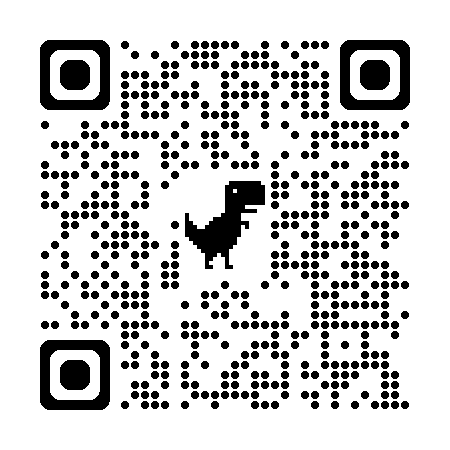
\includegraphics[width=4cm]{qrcode_yoheiyamashita-svg.github.io.png}
\end{center}

\clearpage


\end{document}